\chapter{Seismik}

Das Gebiet der Seismik umfasst die Analyse der Ausbreitung elastischer Wellen in der Erde. Diese Wellen werden an Schichtgrenzen oder Objekten im Untergrund reflektiert, refraktiert und transmittiert. Was genau das bedeutet, wollen wir nach einer Einführung in das Thema seismische Wellen klären.  

\section{Seismische Wellen} 
Man unterscheidet zwischen zwei verschiedenen Wellentypen, den Raum- und den Oberflächenwellen. 
\subsection{Raumwellen}
Raumwellen breiten sich über einen Raum aus, das heißt in unserem Fall, dass sie bis weit unter die Erdoberfläche über einen großen Bereich wirken.

\subsubsection{P-Welle}
Eine P-Welle schwingt parallel zur Ausbreitungsrichtung und ist damit eine Kompressionswelle (Longitudinalwelle). P-Welle ist hierbei die Abkürzung für Primär-Welle, da diese Welle die schnellste Wellenart ist und somit als erstes auftritt.
 
\subsubsection{S-Welle} 
Die S-Welle ist langsamer als die P-Welle und tritt als zweites auf. Daher auch der Name Sekundär-Welle. Es handelt sich bei der S-Welle um eine Scherwelle (Transversalwelle) und der Ausschlag ist senkrecht zur Ausbreitungsrichtung. In Flüssigkeiten treten S-Wellen nicht auf.

\begin{figure}[H]
	\begin{subfigure}[m]{0.5\textwidth}
		\centering
		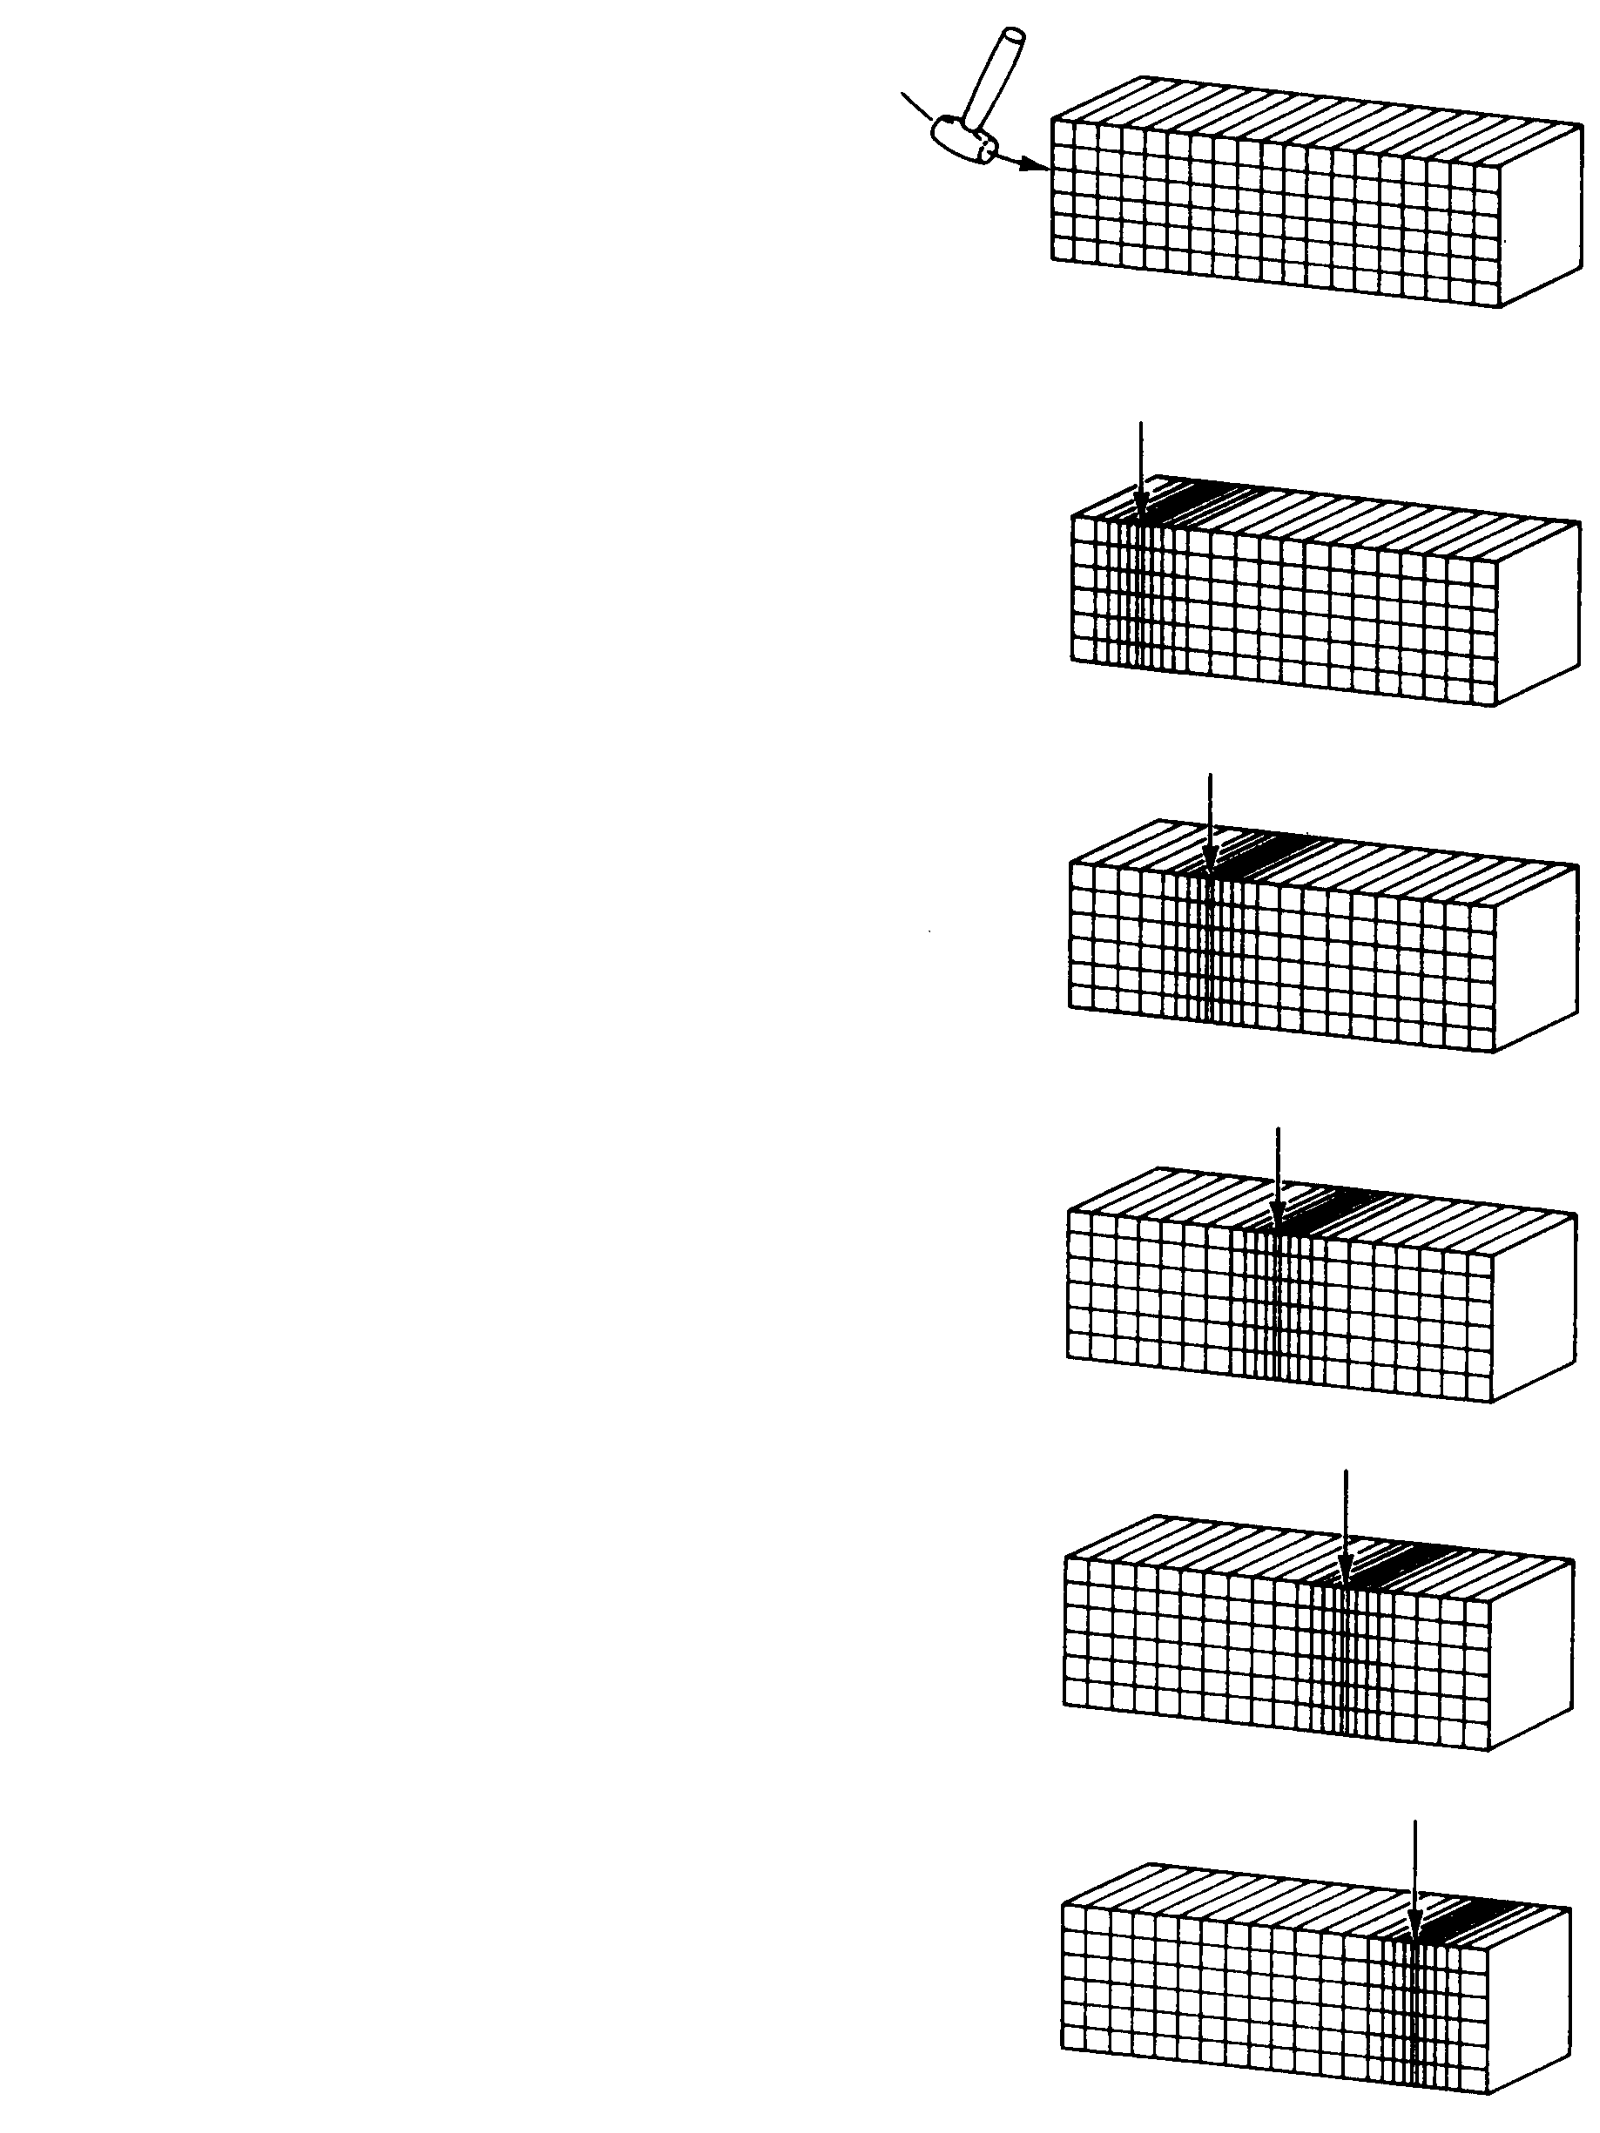
\includegraphics[scale = 0.3]{SeismikBilder/PWelle}
		\caption*{P-Welle}
	\end{subfigure}
	\begin{subfigure}[m]{0.5\textwidth}
		\centering
		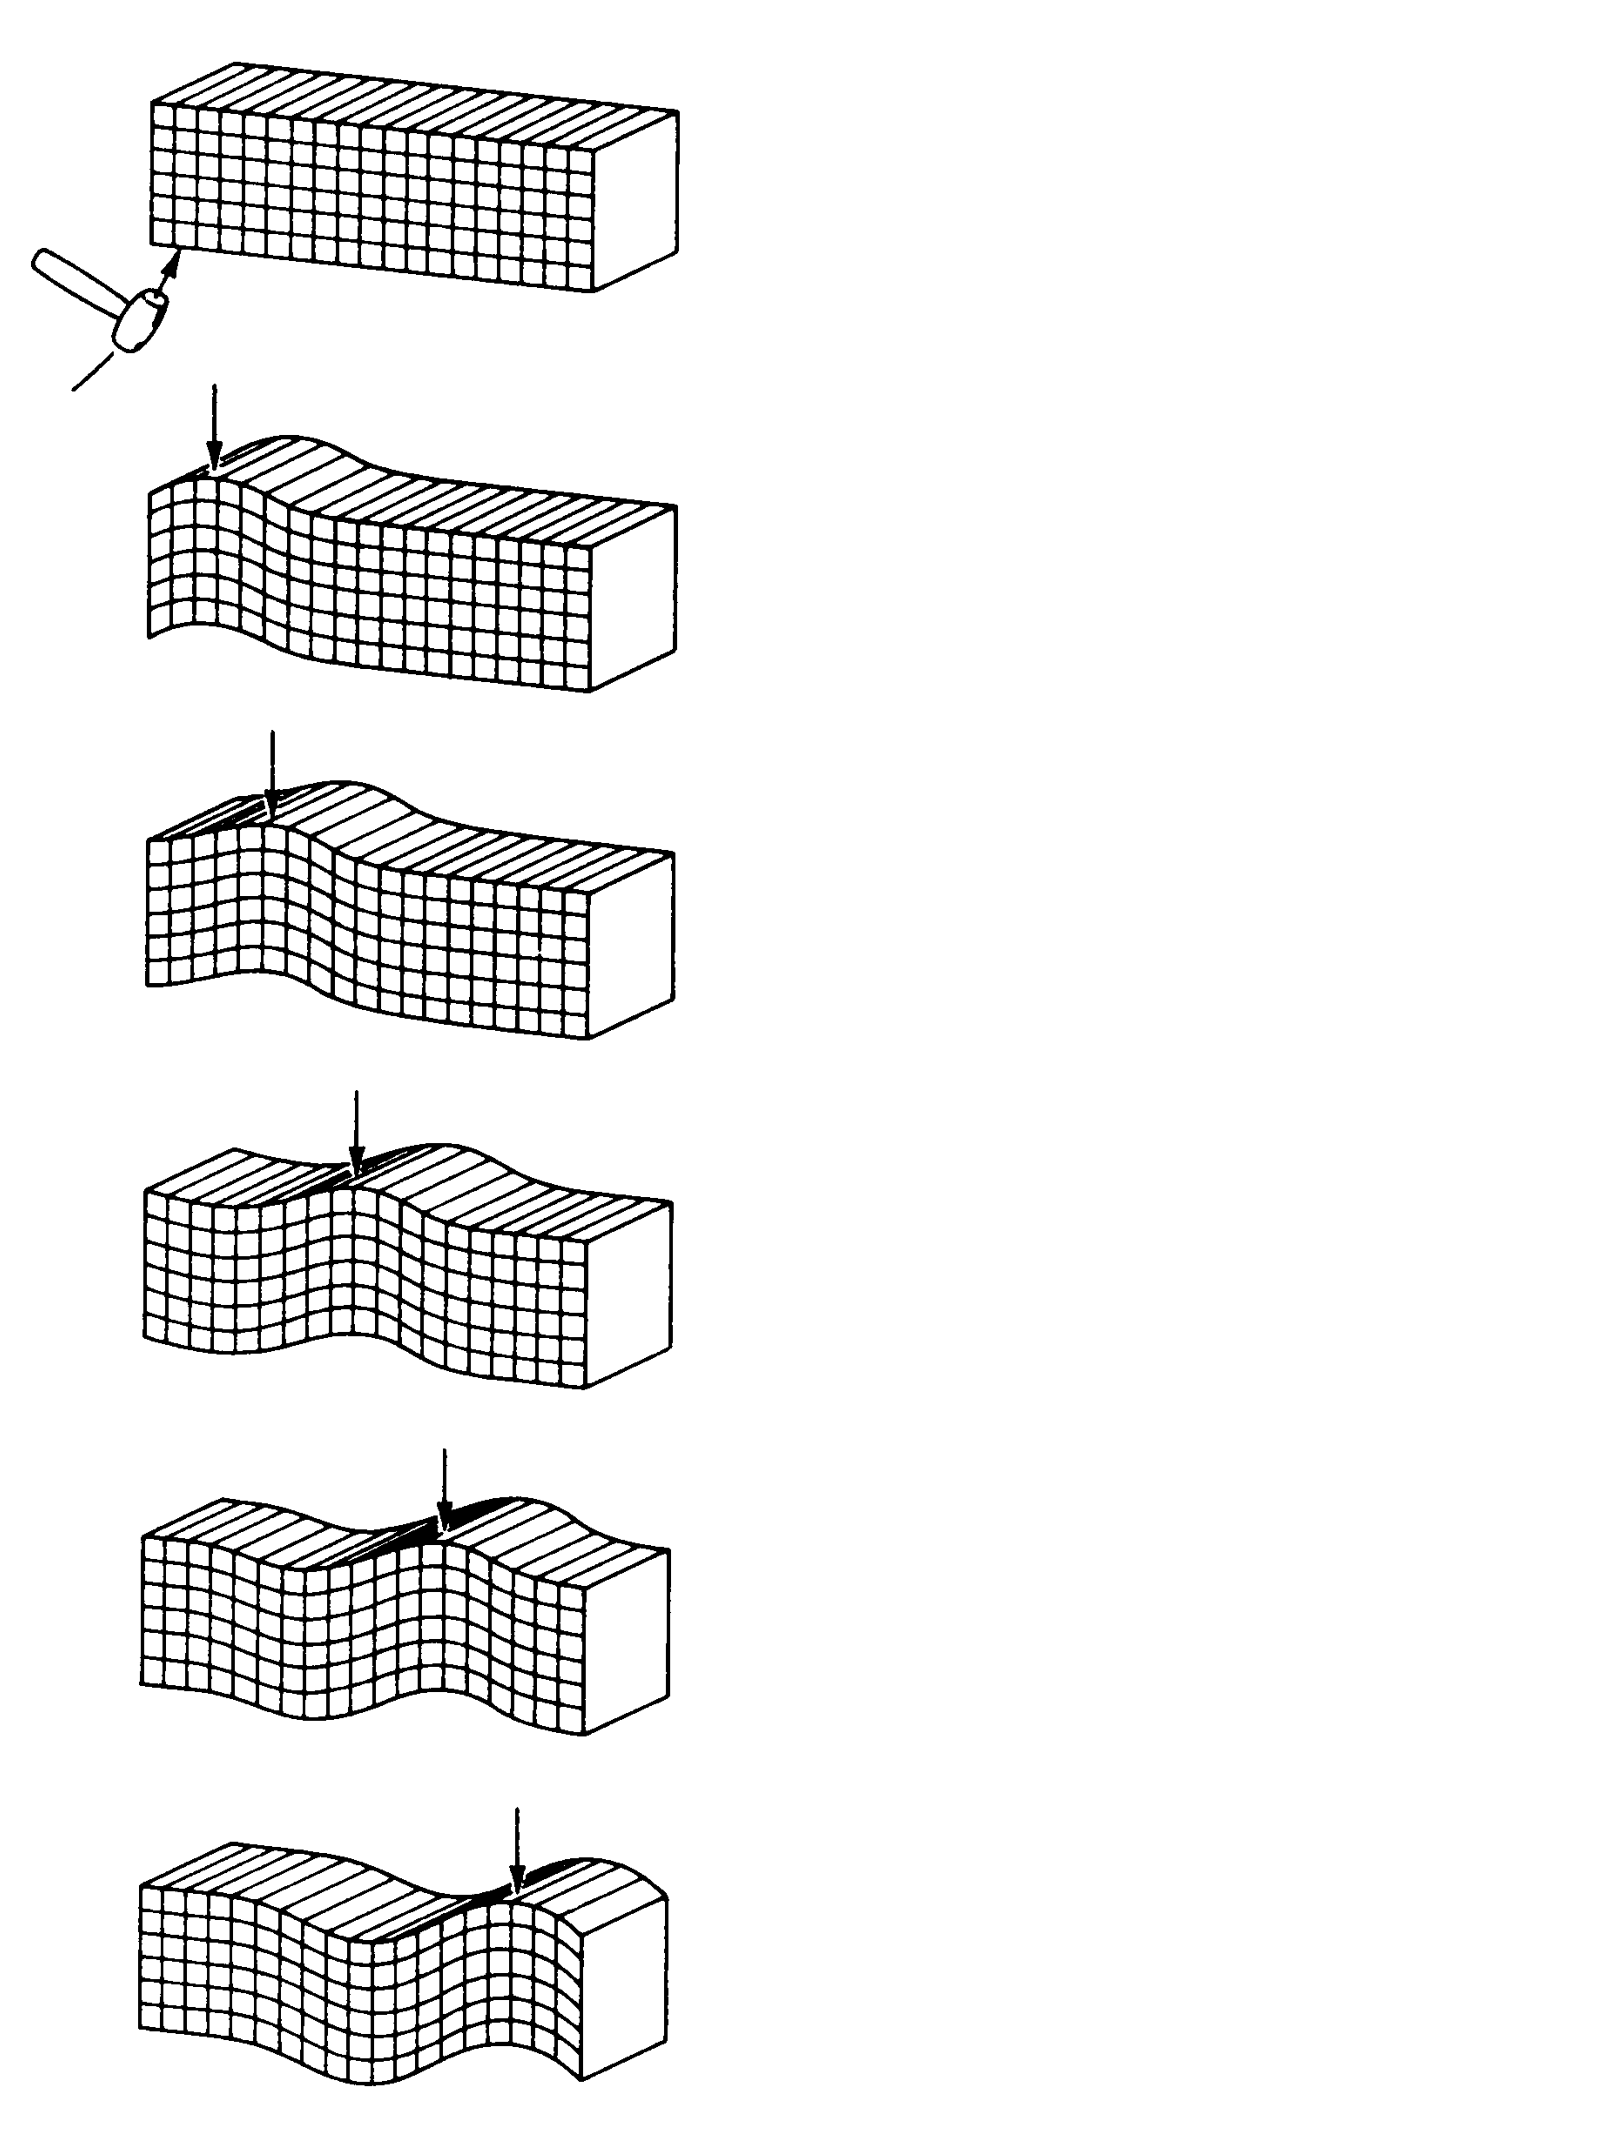
\includegraphics[scale = 0.3]{SeismikBilder/SWelle}
		\caption*{S-Welle}
	\end{subfigure}
\end{figure}

\subsection{Oberflächenwellen}
Wie der Name schon sagt, wirken diese Wellen an der Oberfläche. Allerdings wirken auch sie bis weit in die Tiefe. Die Amplitude, also die Stärke der Welle, nimmt jedoch mit der Tiefe exponentiell ab. 

\subsubsection{Rayleigh-Welle}
Die Rayleigh-Welle ist eine Mischung aus P- und S-Welle, weshalb die Bodenbewegung elliptisch ist. Ist die Bewegung im Uhrzeigersinn, spricht man von retrograder Bewegung, bei Gegenuhrzeigersinn von prograder Bewegung.

Trotz exponentieller Abnahme der Amplitude sind bei starken Erdbeben Schwingungen bis zum Erdkern möglich.


\begin{figure}[H]
	\begin{subfigure}[m]{0.5\textwidth}
		\centering
		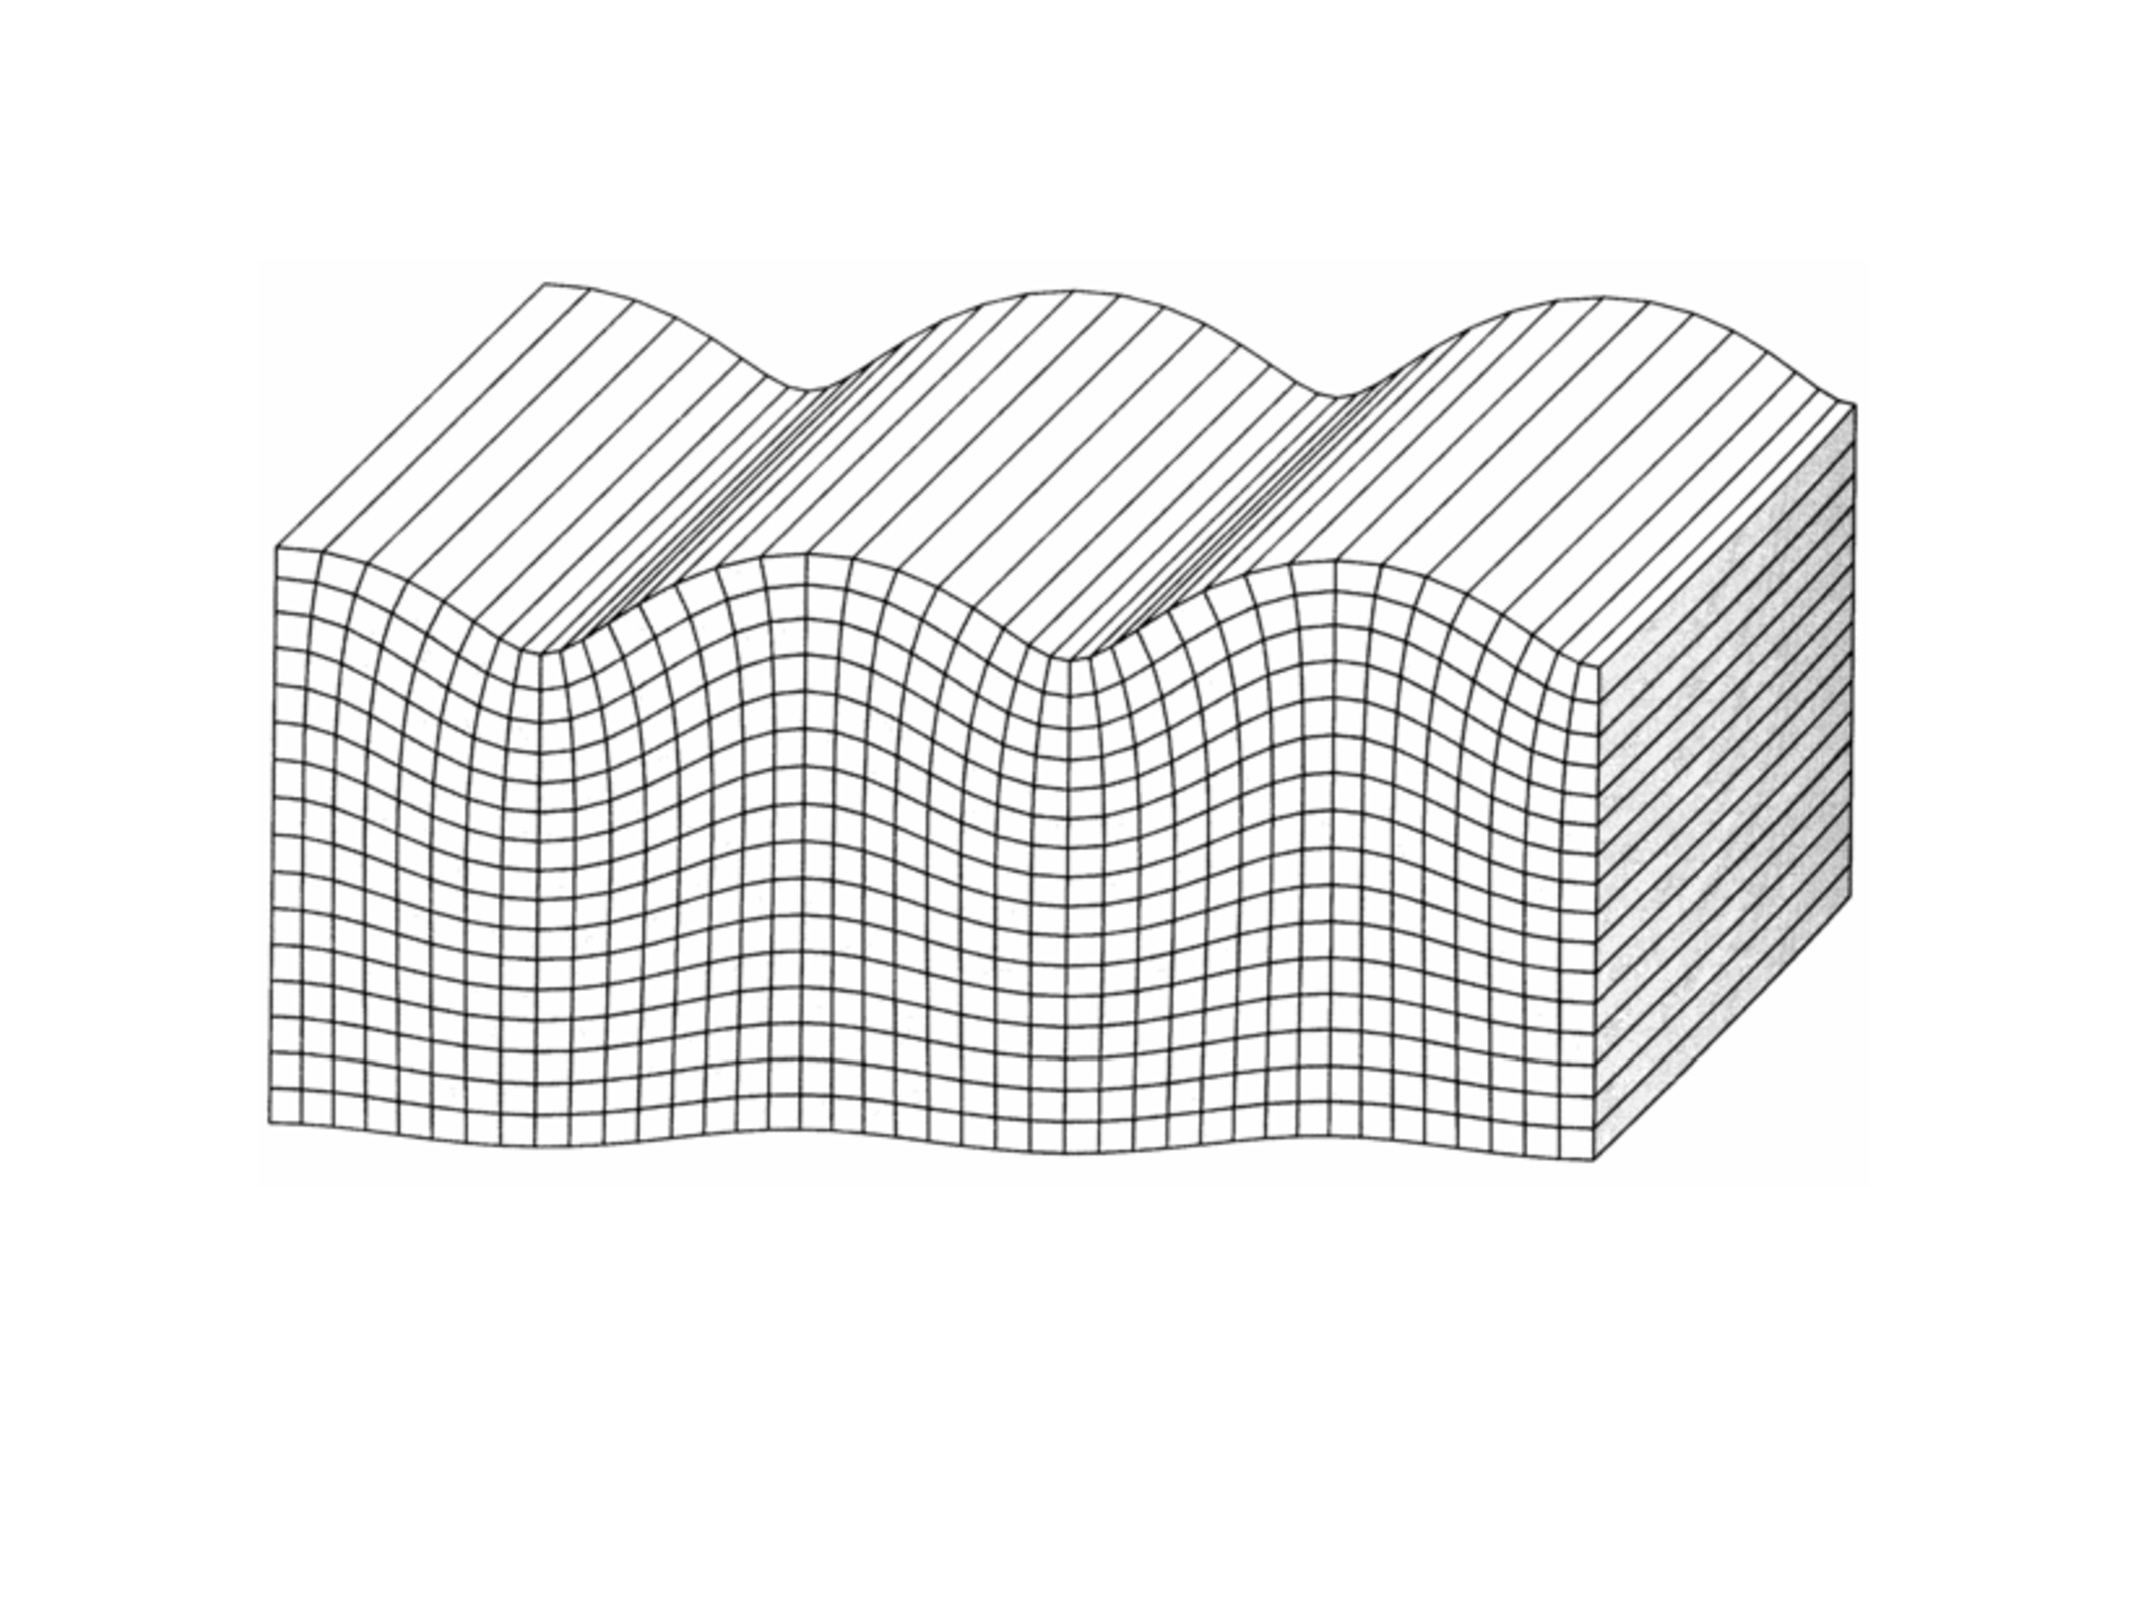
\includegraphics[scale = 0.2]{SeismikBilder/RayleighWelle}
	\end{subfigure}
	\begin{subfigure}[m]{0.5\textwidth}
		\centering
		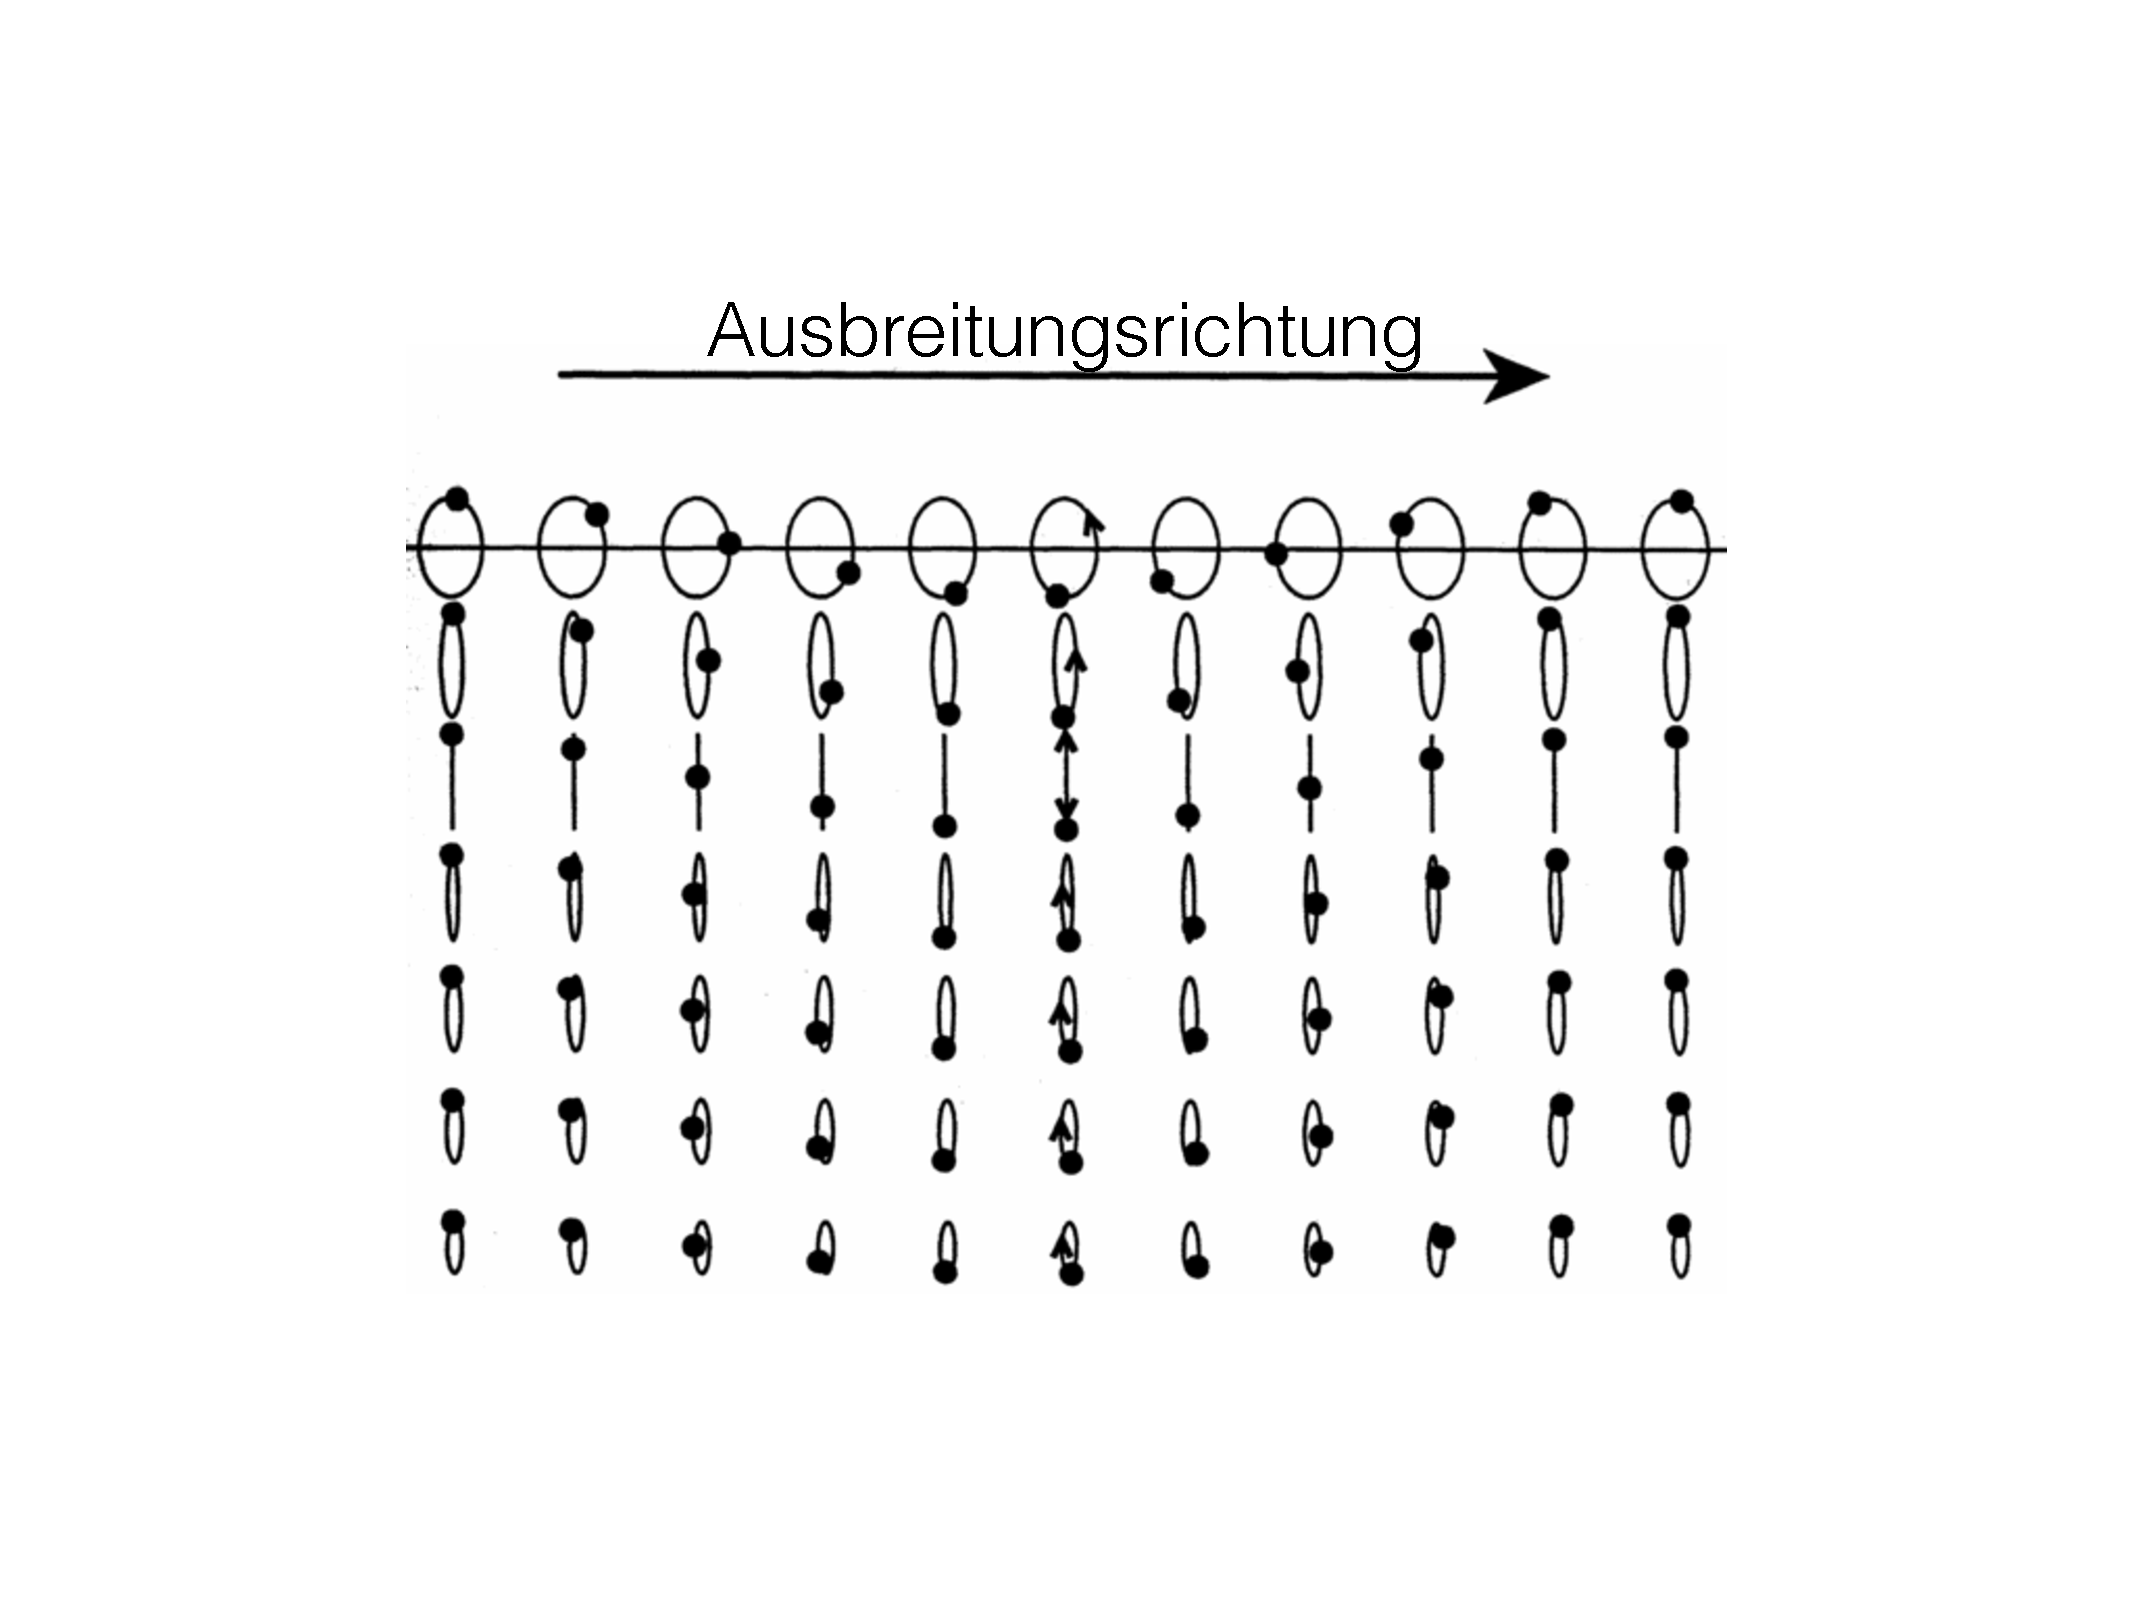
\includegraphics[scale = 0.2]{SeismikBilder/BodenbewegungRayleigh}
	\end{subfigure}
	\caption*{Bodenbewegung einer Rayleigh-Welle \textsl{Quelle: Shearer}}
\end{figure}

\subsubsection{Love-Welle}
Eine Love-Welle ist eine S-Welle mit Schwingungsrichtung parallel zur Erdoberfläche.

\begin{figure}[H]
	\centering
	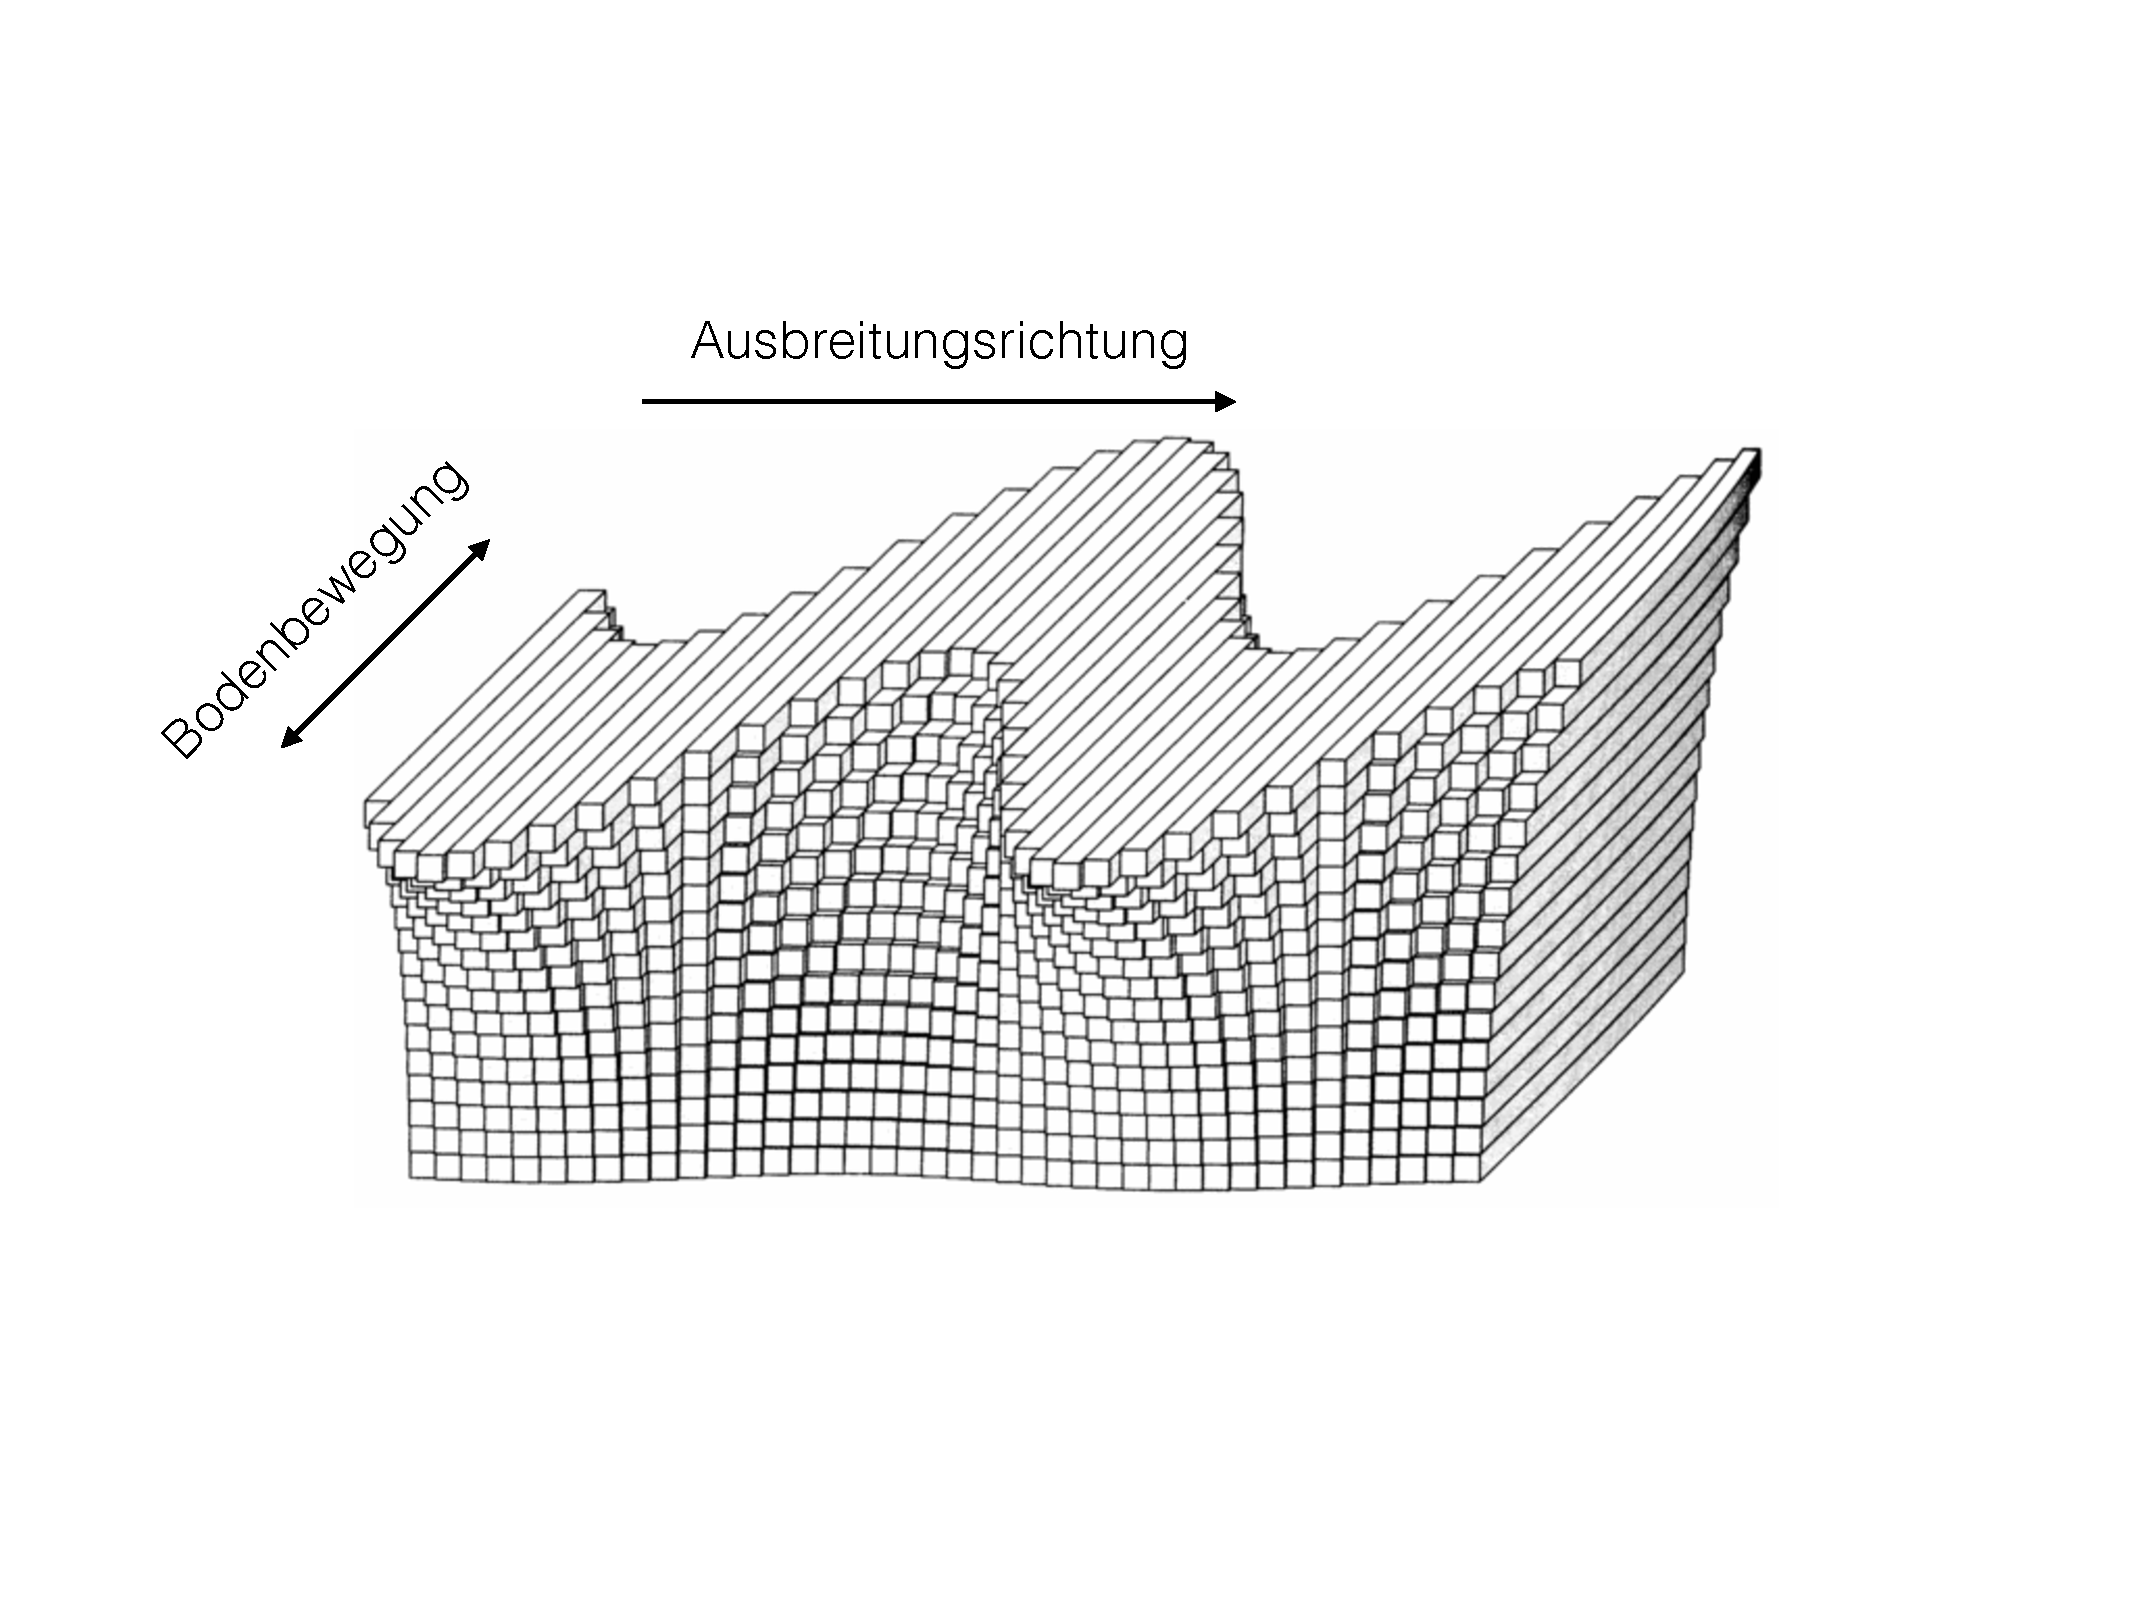
\includegraphics[width = \textwidth]{SeismikBilder/LoveWelle}
	\caption*{\textsl{Quelle: Shearer}}
\end{figure}


\section{Ausbreitungsgeschwindigkeiten}
Die Geschwindigkeiten der Wellen sind abhängig von den elastischen Moduln. Diese Moduln sind Konstanten, die abhängig von den Eigenschaften des Materials sind.
Uns interessieren dabei besonders zwei davon: \begin{description}
	\item[Kompressionsmodul $K$:] Dieser Wert gibt an, wie stark man einen Körper zusammendrücken muss, bis er sein Volumen verändert.
	\item[Schermodul $\mu$:] Der Wert des Schermoduls gibt den Widerstand des Materials gegen Scherkräfte an.\end{description}

Beide Werte werden in Pascal (\si{Pa}) angegeben.


Um die Wellengeschwindigkeit von P- und S-Welle berechnen zu können, müssen die elastischen Moduln $K$ und $\mu$, sowie die Dichte $\rho$ des Untergrunds bekannt sein.

\subsection{Geschwindigkeit P-Welle}
\begin{equation*}
	v_{\text{p}} = \sqrt{\frac{K + \frac{4}{3} \mu}{\rho}}
\end{equation*}
Ein wichtiger Faktor für die Geschwindigkeit einer P-Welle ist der Sättigungsgrad der Poren mit Wasser. Ab einem Sättigungsgrad von 85\% steigt die Geschwindigkeit stark an.

\subsection{Geschwindigkeit S-Welle}
\begin{equation*}
	v_{\text{s}} = \sqrt{\frac{\mu}{\rho}}
\end{equation*}
In Flüssigkeiten gilt $\mu = 0$, da S-Wellen hier nicht auftreten. \par

Um ein Gefühl für die Geschwindigkeit einer Bodenwelle zu bekommen seien hier Werte einer P-Welle genannt. 

\begin{tabular}{ll}
	\textbf{Material} & \textbf{Typische Geschwindigkeit}\\
	Luft & 0,33\,\si{km/s} \\
	Sand, Verwitterungsboden & 0,3 -- 1,5 \si{km/s} \\
	Wasser & 1,5\,\si{km/s}\\
	Eis & 3,0 -- 4,0\,\si{km/s}\\
	Sandstein & 1,5 -- 4,3\,\si{km/s}\\
	Kalkstein/Dolomit & 4,0 -- 4,5\,\si{km/s}\\
	Steinsalz & 4,0 -- 5,5\,\si{km/s}\\
	Granit & 5,8 -- 6,2\,\si{km/s}\\
	Gabbro & 6,4 -- 7,6\,\si{km/s}\\
	Peridotit & 7,8 -- 8,4\,\si{km/s}
\end{tabular}

\subsection{Poisson-Zahl}
Die Poisson-Zahl $\sigma$ beschreibt das Verhältnis der Quer- zur Längsverformung. Dieses Verhältnis erlaubt Aussagen über das Verhalten einer Materie bei Belastung in eine Richtung. Bei einer Flüssigkeit beispielsweise bleibt das Volumen bei Quetschung erhalten, da die Flüssigkeit einfach zur Seite ausweicht. $\sigma$ ist in diesem Fall 0,5. Dies ist der höchste Wert, den die Poisson-Zahl annehmen kann. Eine Flüssigkeit ist demnach ideal plastisch.
Festkörper können bei Quetschung und Dehnung aufgrund ihrer elastischen Eigenschaften nicht instantan reagieren und zur Seite ausweichen. $\sigma$ ist hier im Bereich um 0,25. Besonders ist $\sigma$ von Quarz. Hier beobachtet man eine negative Poisson-Zahl. Das liegt daran, dass Quarz sich lateral zusammenzieht wenn eine axiale Spannung anliegt.

\begin{figure}[H]
	\centering
	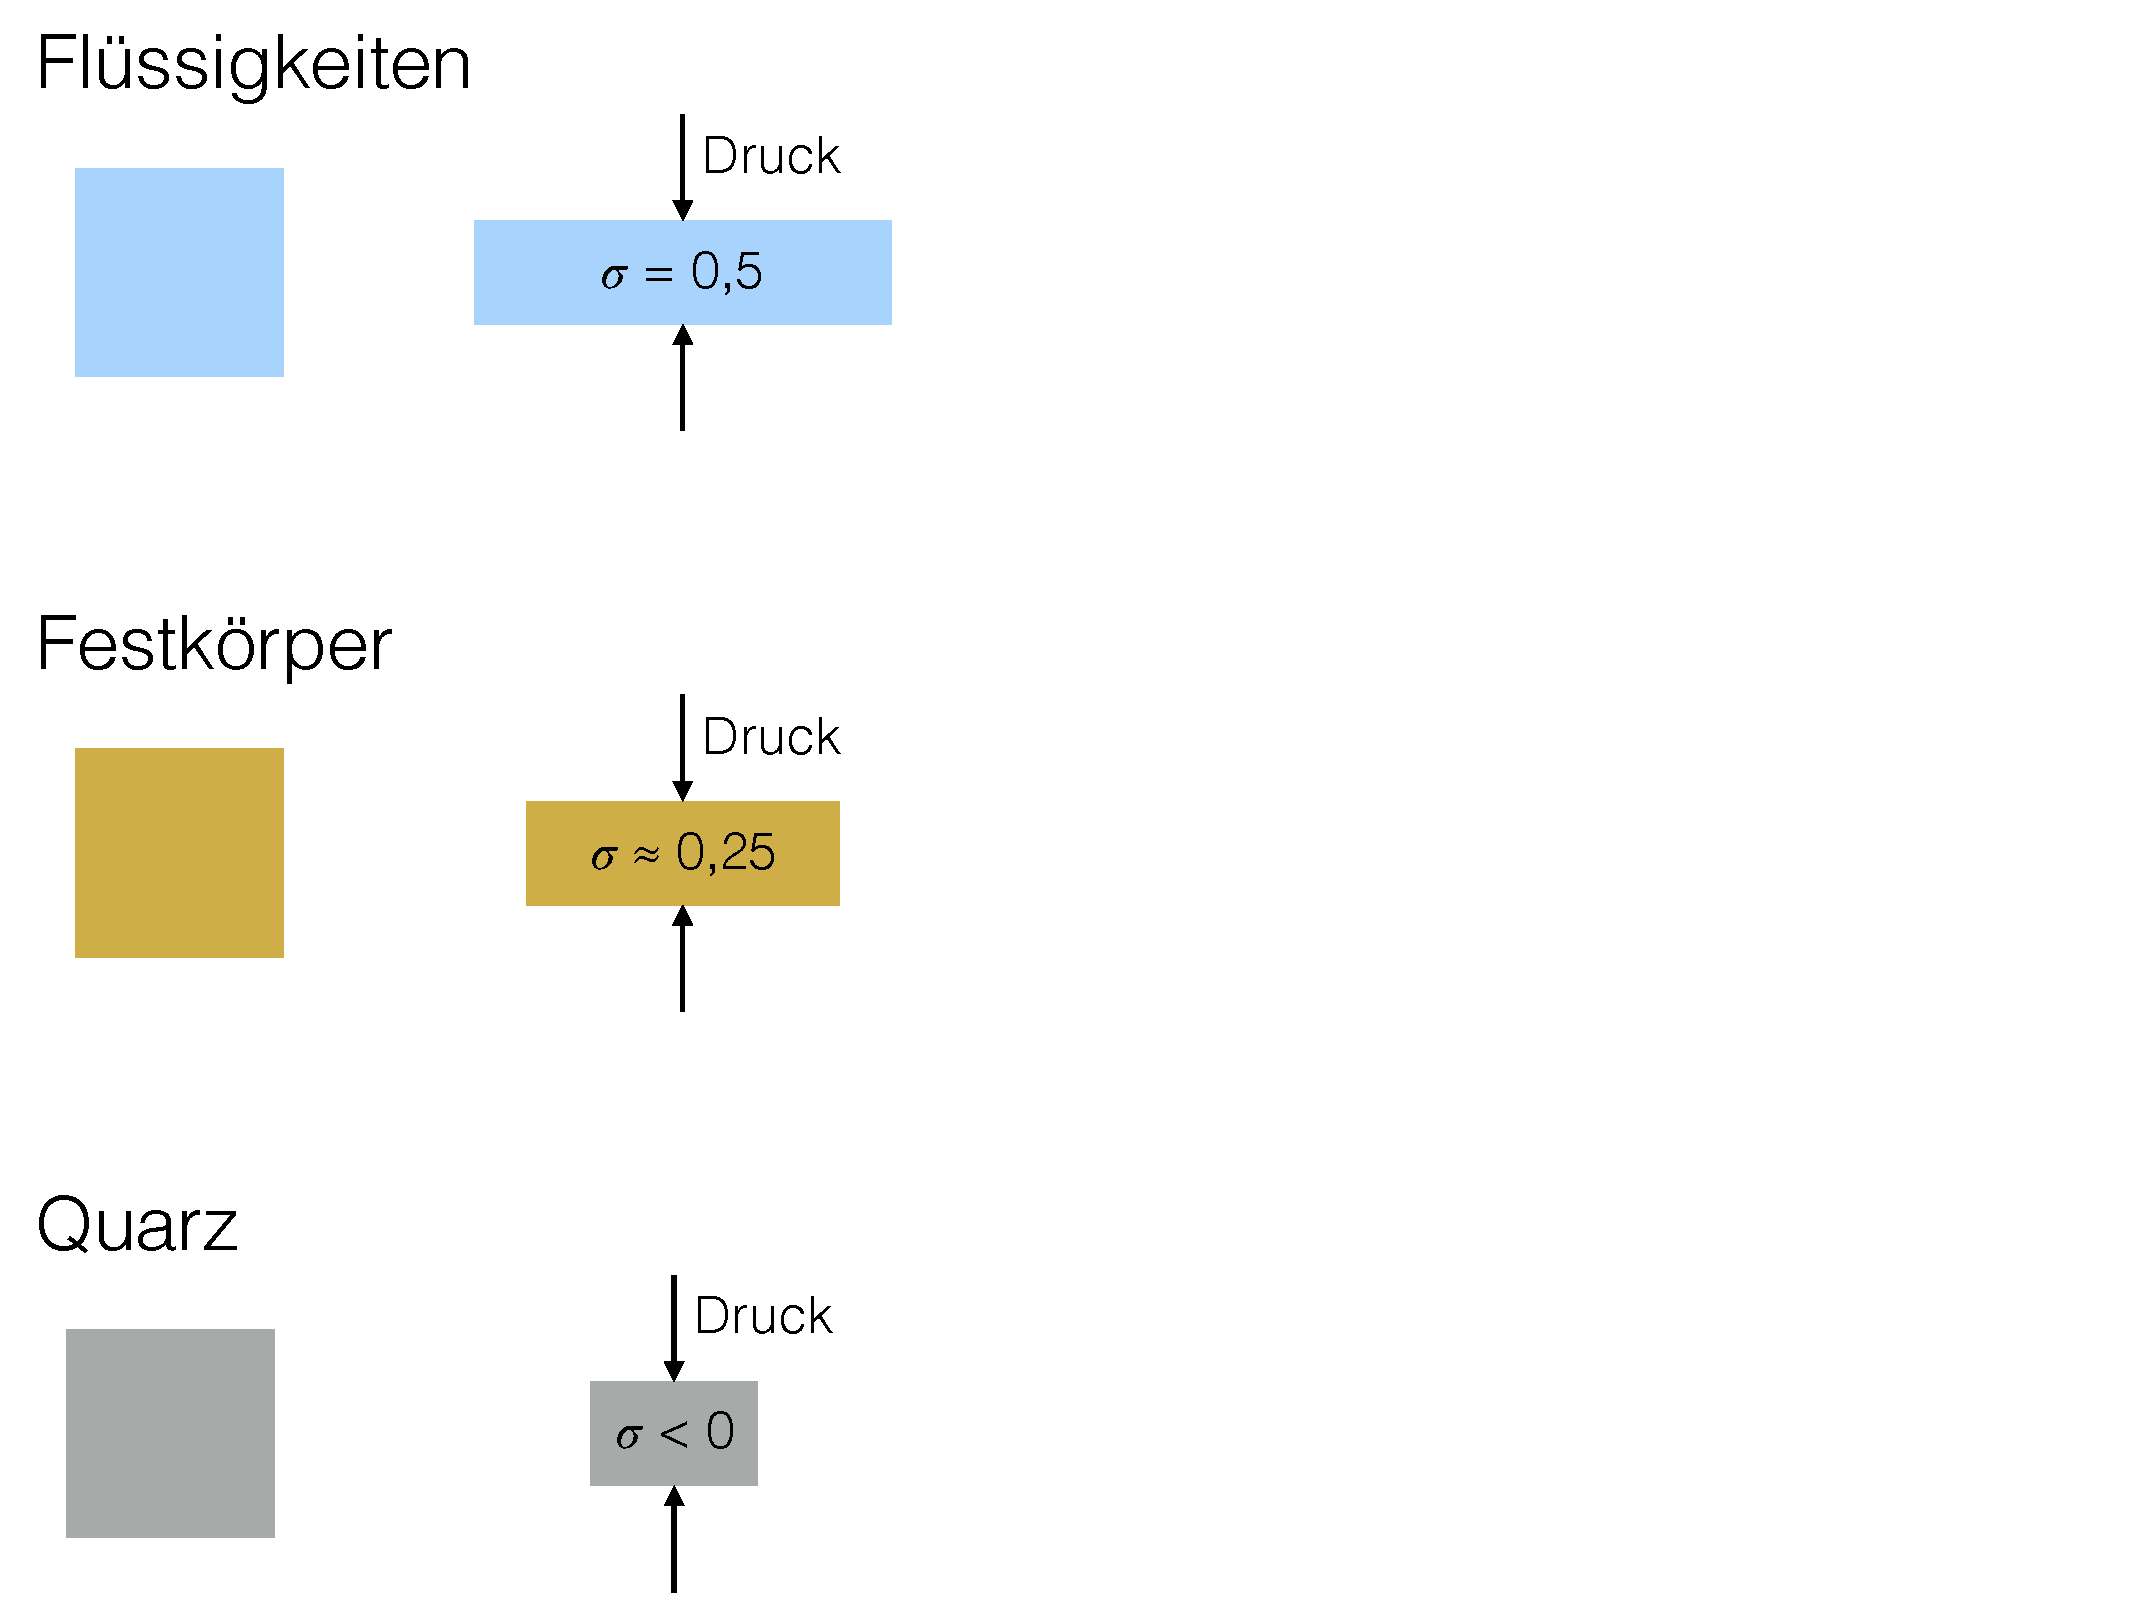
\includegraphics[scale = 0.3]{SeismikBilder/PoissonZahl}
\end{figure}


Die Poisson-Zahl berechnet sich zu: 
\begin{equation*}
	\sigma = \frac{\left( \frac{v_{\text{p}}}{v_{\text{s}}} \right)^2 - 2}{2 \cdot \left( \frac{v_{\text{p}}}{v_{\text{s}}} \right)^2 - 2} \qquad \text{mit } -1 < \sigma \leq 0,5 
\end{equation*}



\section{Wellenausbreitung}
Eine Welle wird an einer Schichtgrenze reflektiert, refraktiert und transmittiert.\begin{description}
	\item[Reflexion:] Ein Teil der Welle wird an der Schichtgrenze ins obere Medium zurückgeworfen.
	\item[Transmission:] Ein Teil der Welle wird uns untere Medium gebrochen. 
	\item[Refraktion:] Ein Teil der Welle läuft entlang der Schichtgrenze.
\end{description}


Bevor wir genauer auf die einzelnen Begriffe eingehen, schauen wir uns einmal die zu Grunde liegende physikalische Überlegung an.


\subsection{Huygen'sches Prinzip}
Jeder Punkt einer Wellenfront ist der Ausgangspunkt einer neuen Elementarwelle (Kreis- bzw. Kugelwelle). Diese neuen Wellen breiten sich mit der gleichen Geschwindigkeit aus wie die ursprüngliche Welle. Die neue Wellenfront ist dann die Einhüllende der einzelnen Elementarwellen.

\begin{figure}[H]
	\centering
	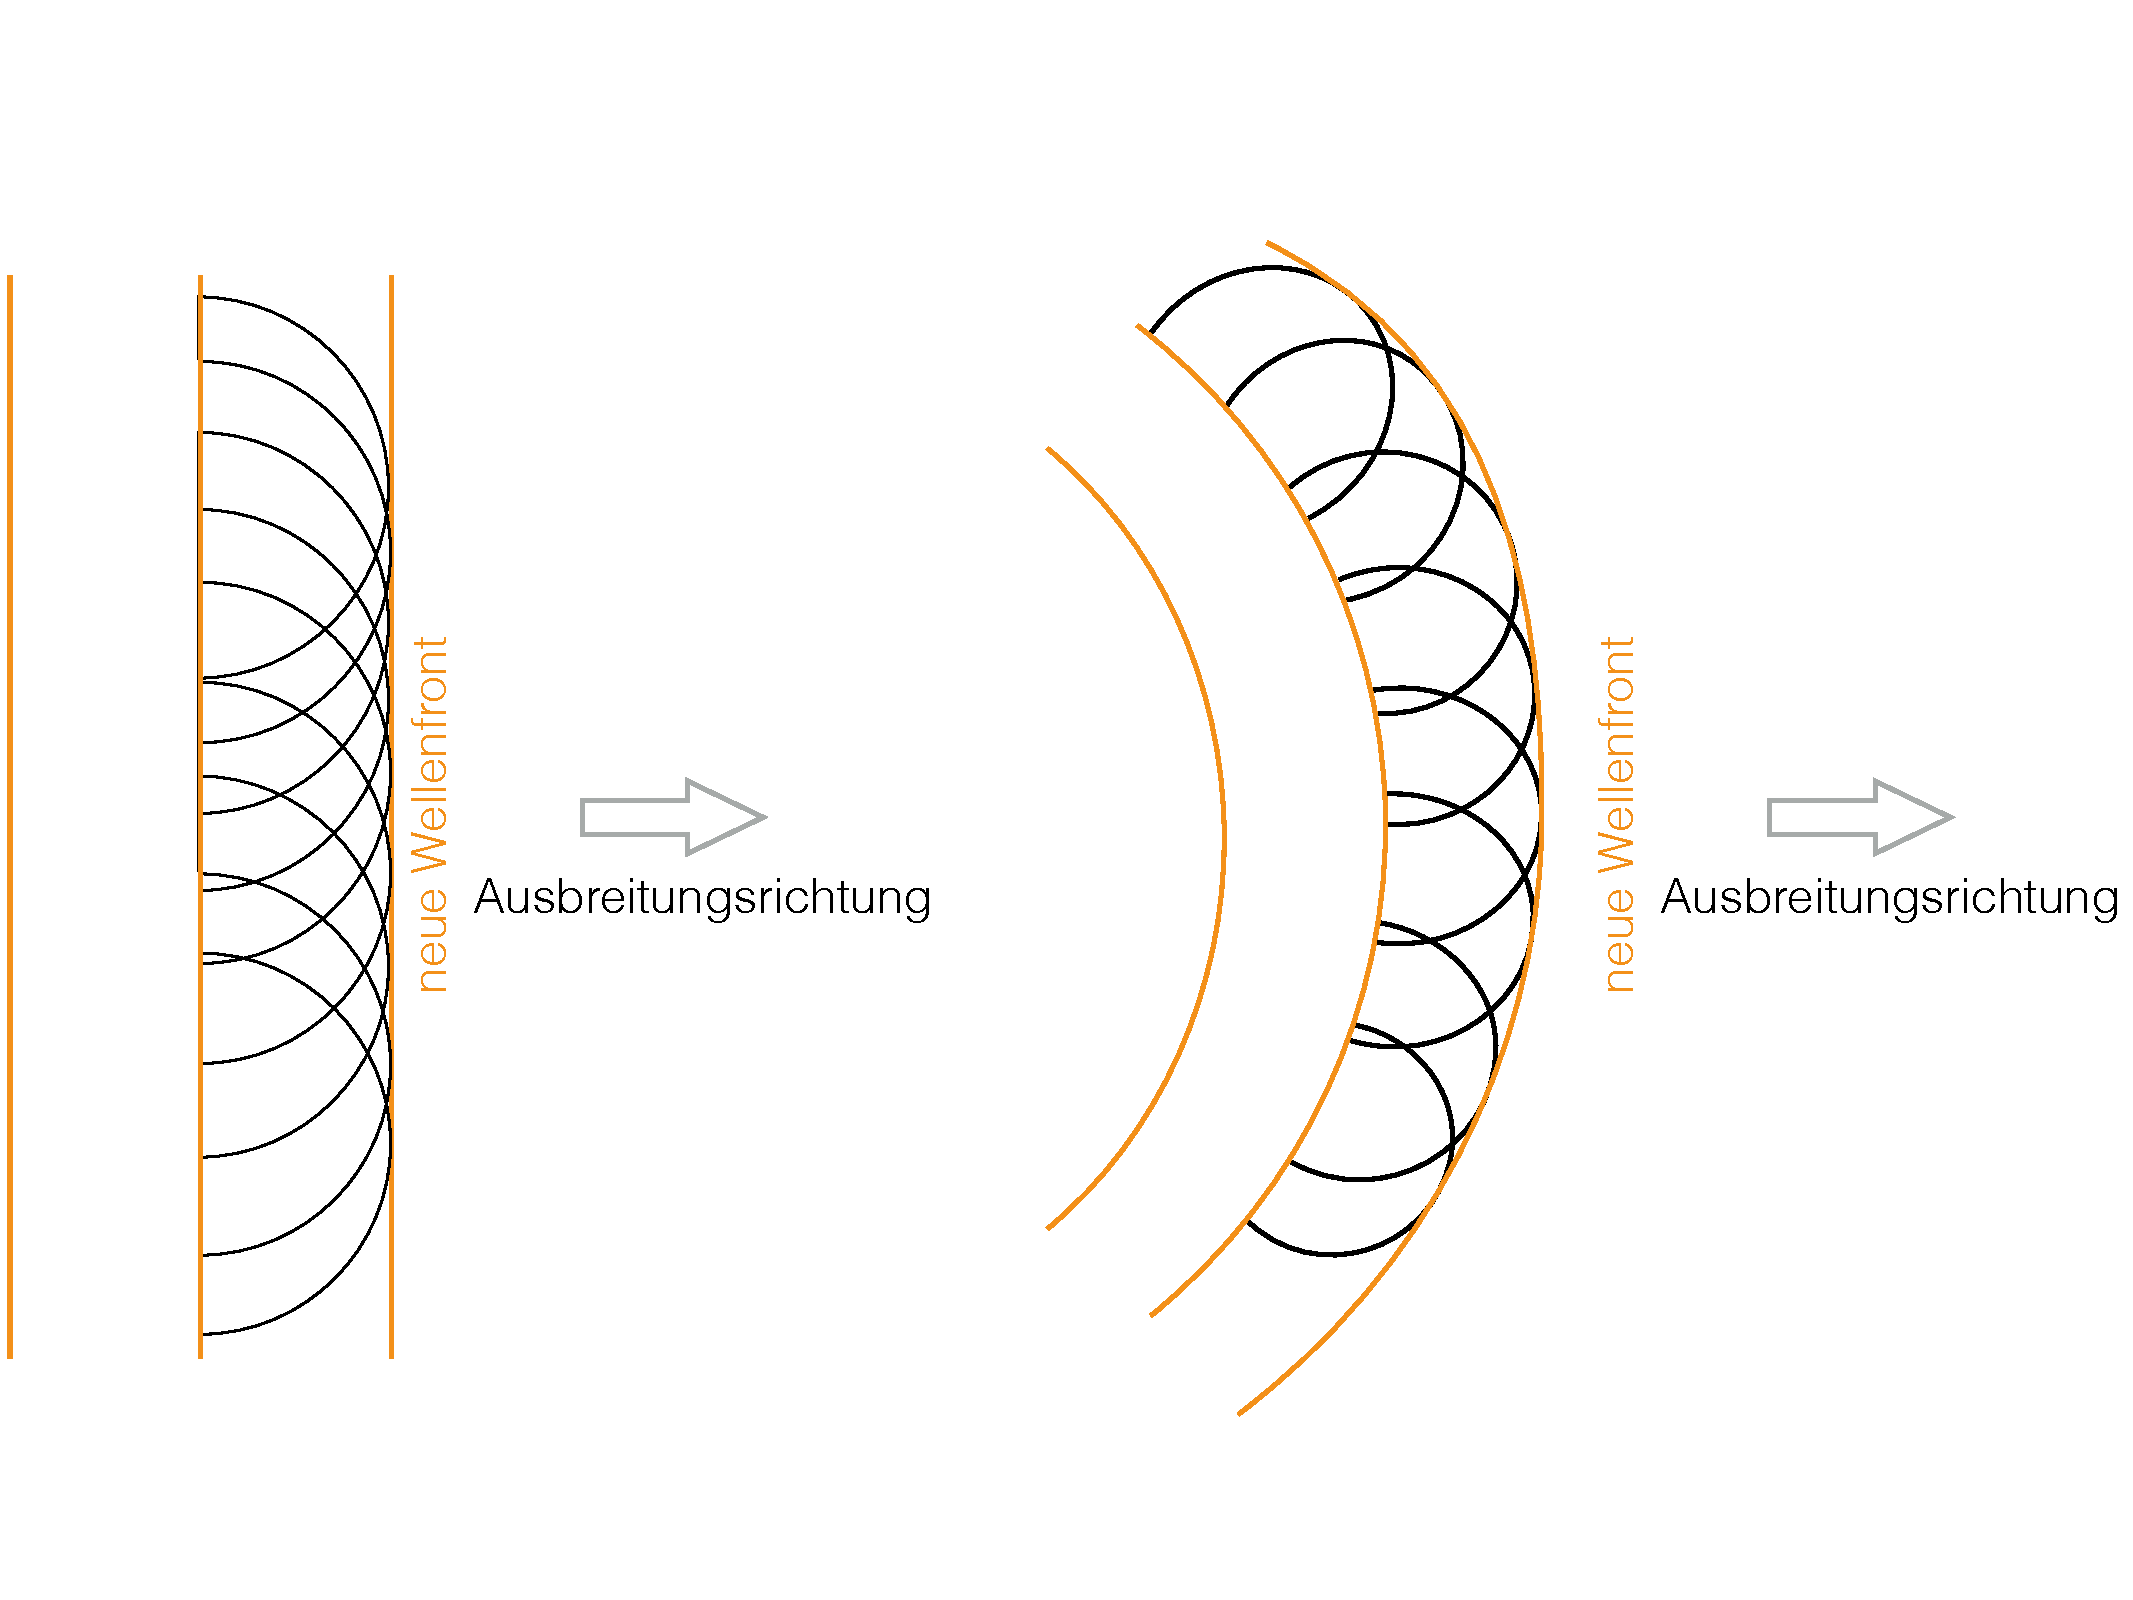
\includegraphics[width = \textwidth]{SeismikBilder/HuygensPrinzip1}
\end{figure}

Diese Grafik zeigt das Huygen'sche Prinzip für den Fall, dass die Welle ungehindert fortlaufen kann. Was aber passiert im Falle einer Reflexion oder Brechung an einer Schichtgrenze? 
Die zwei Grafiken unten zeigen, dass sich das Huygen'sche Prinzip einfach übertragen lässt. 

\begin{figure}[H]
	\centering
	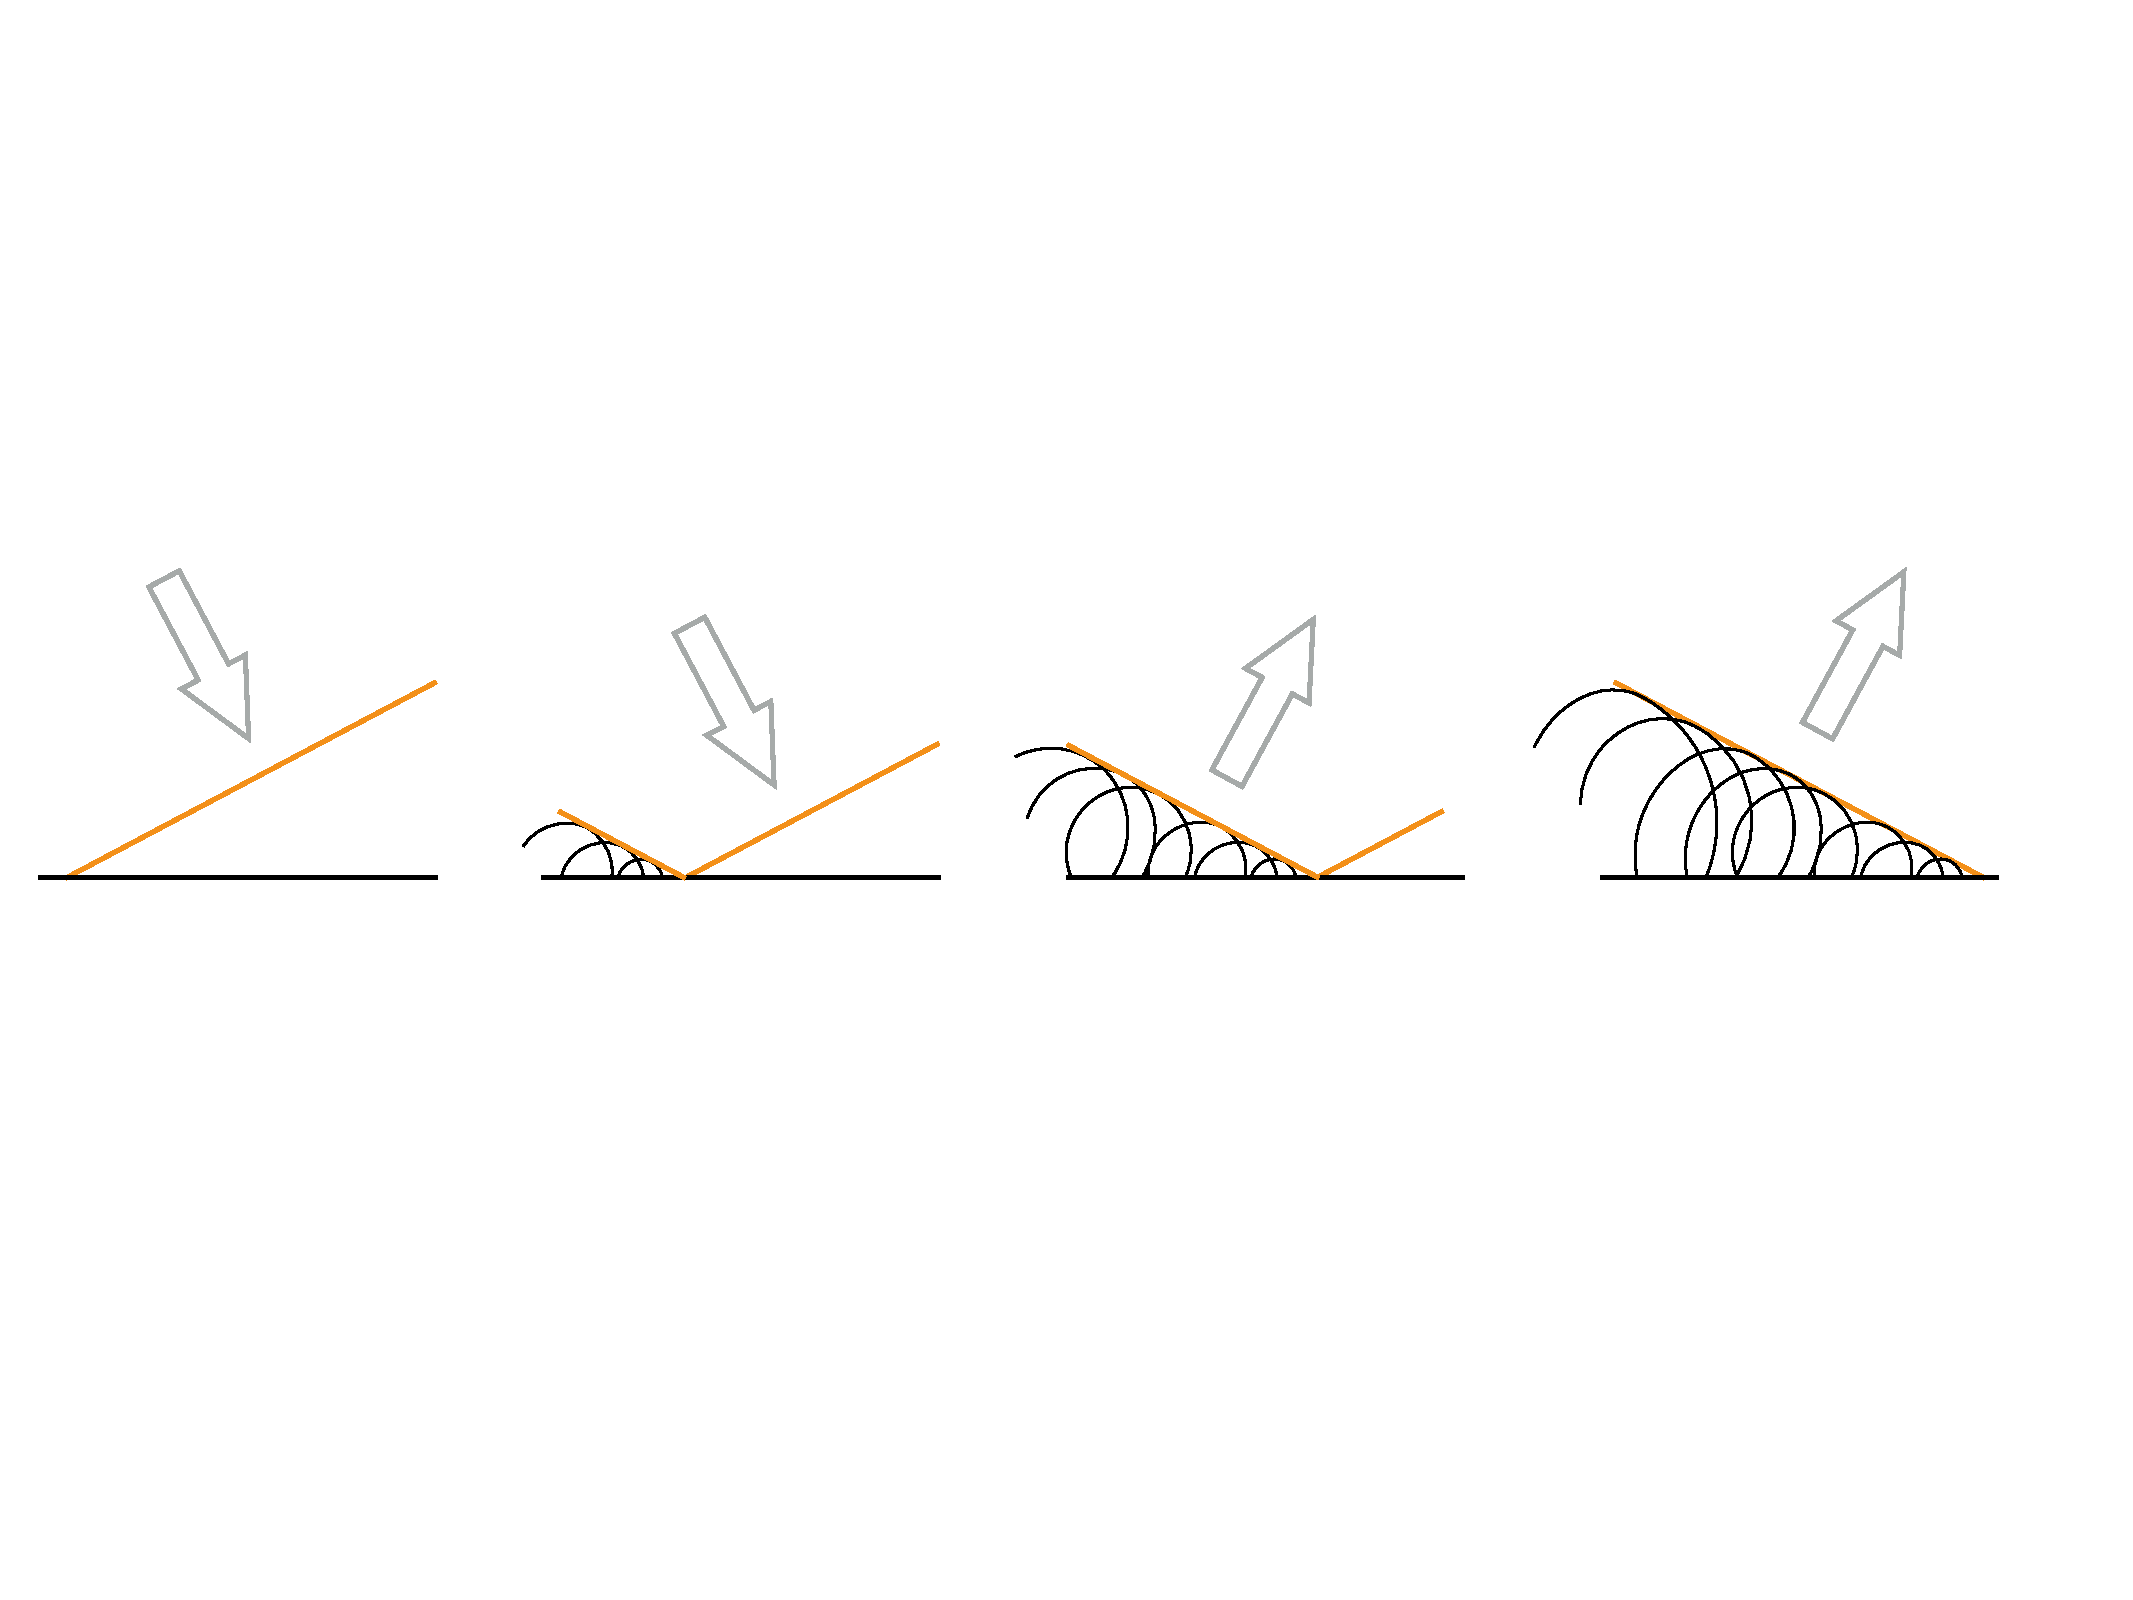
\includegraphics[width = \textwidth]{SeismikBilder/HuygensReflexion}
	\caption*{Reflexion}
\end{figure}

\begin{figure}[H]
	\centering
	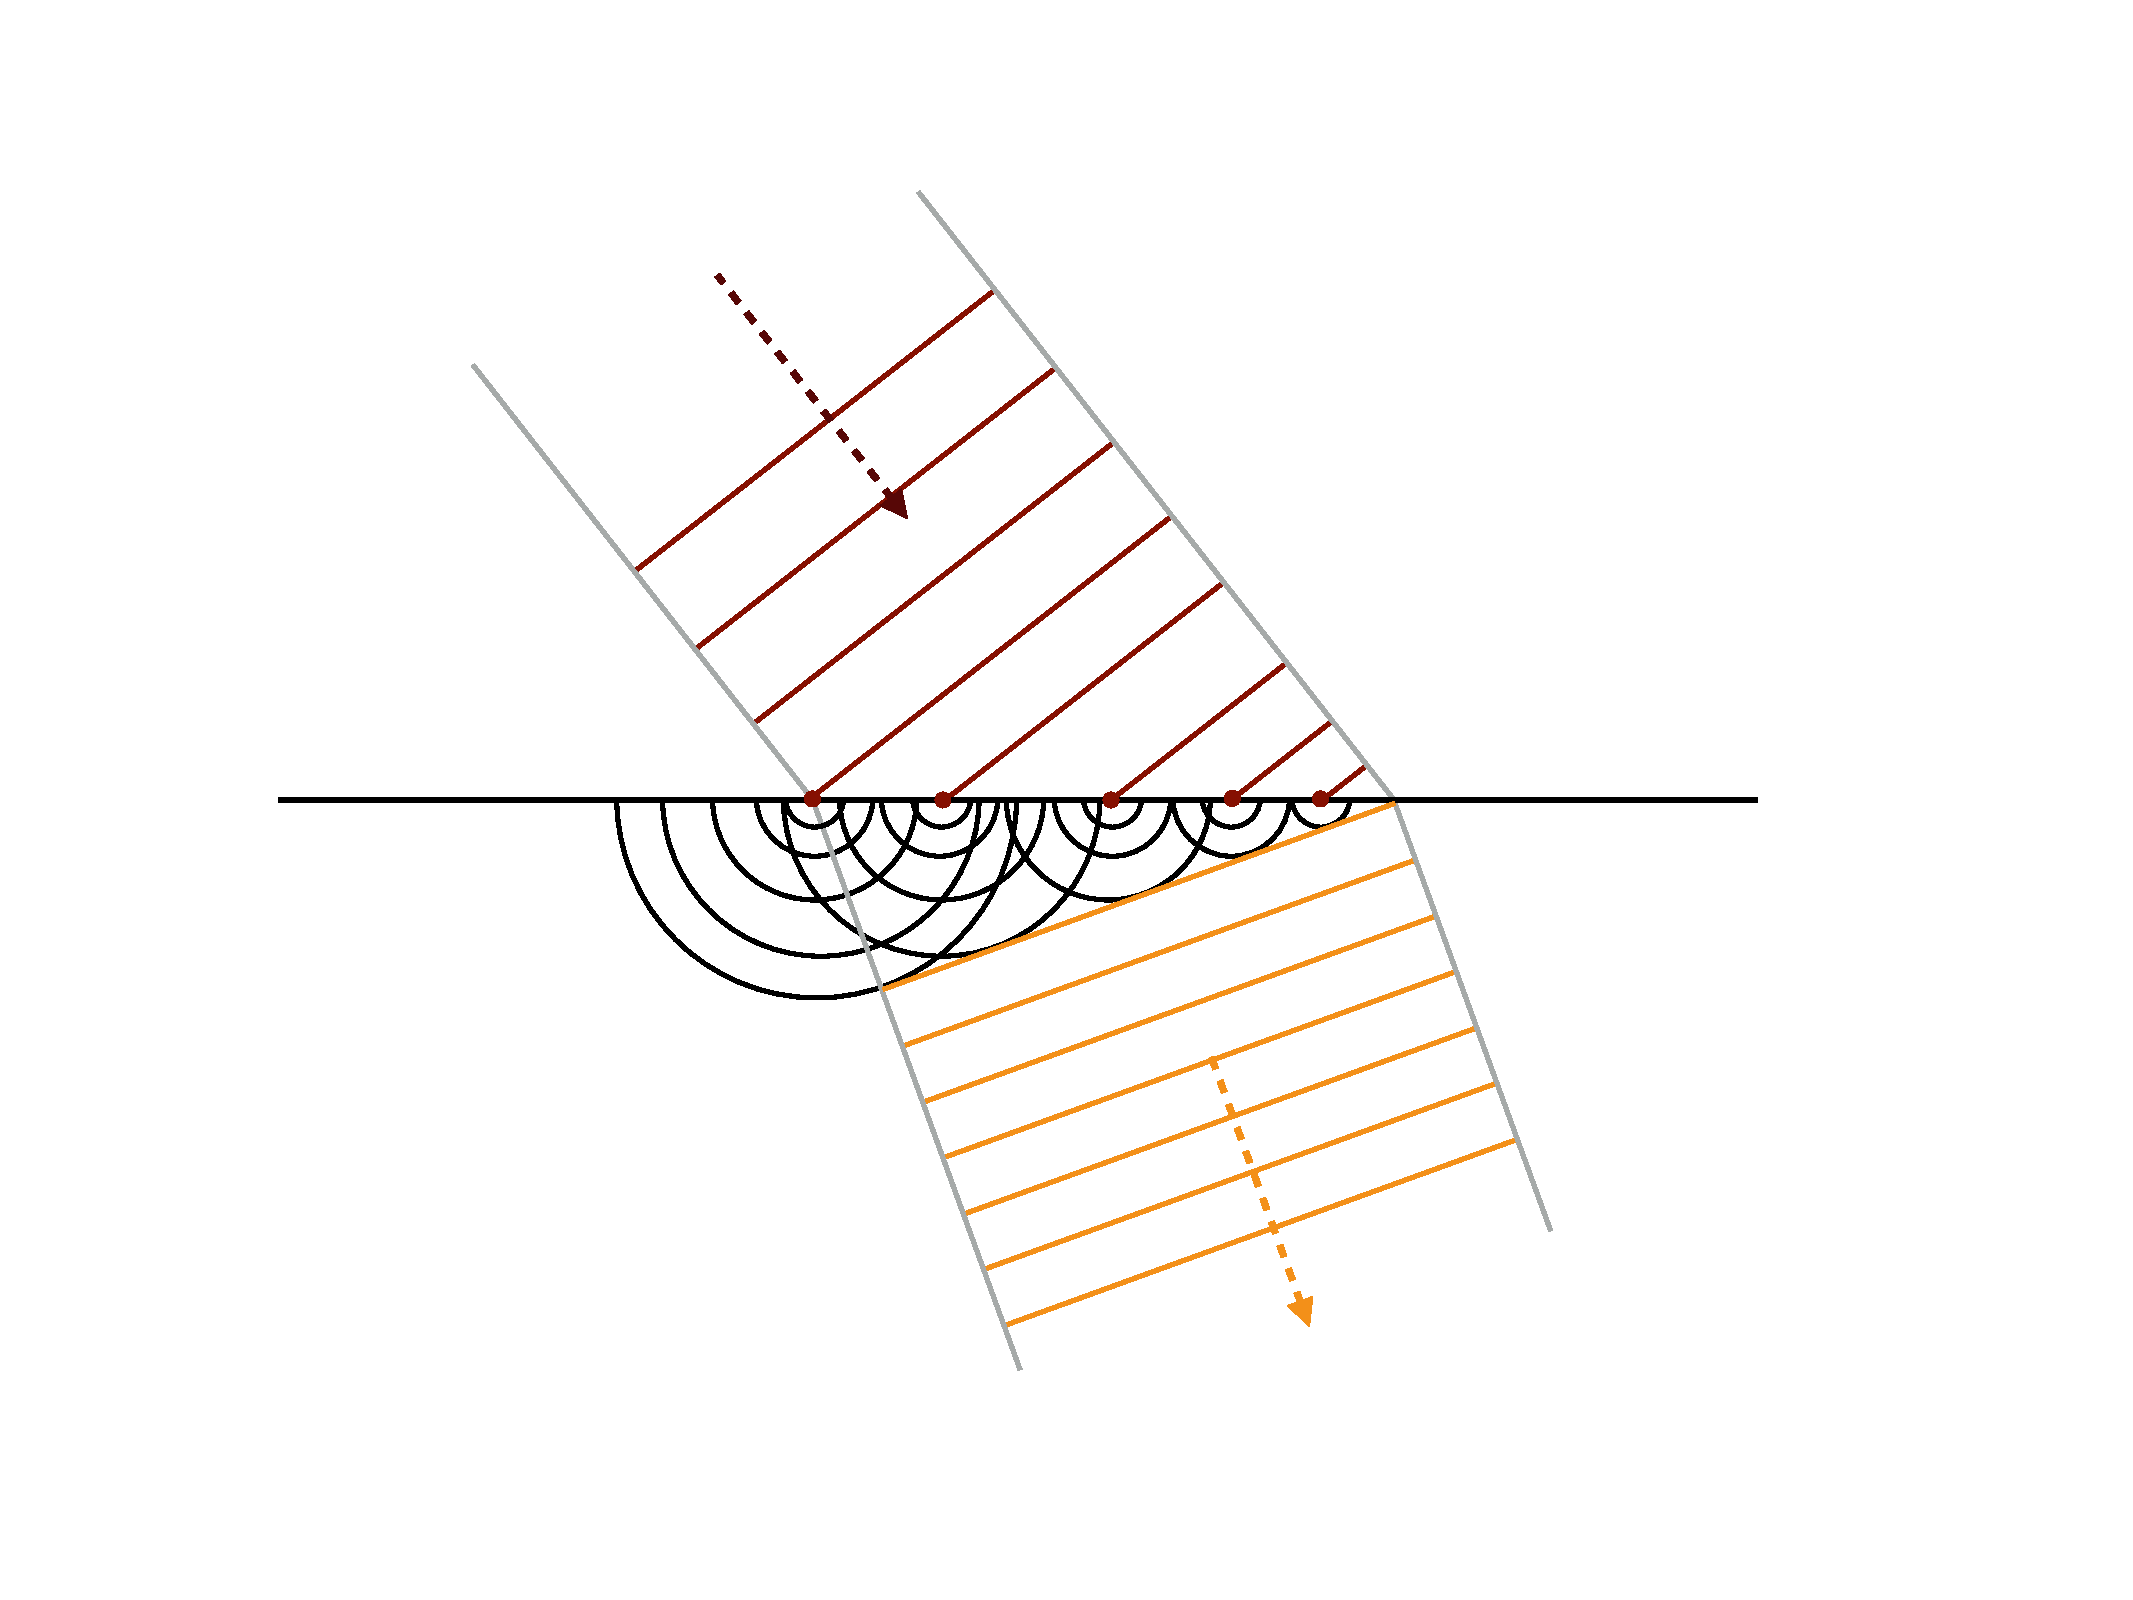
\includegraphics[width = \textwidth]{SeismikBilder/HuygensBrechung}
	\caption*{Brechung}
\end{figure}


\section{Brechungsgesetze}
Trifft eine Welle auf eine Schichtgrenze im Untergrund, wird sie gebrochen. Die Winkel, mit dem die Welle auftrifft, bzw. abgelenkt wird lässt sich einfach berechnen mit Hilfe des \textbf{Snellius'schen Brechungsgesetz}:

\begin{figure}[H]
	\begin{subfigure}[m]{0.5\textwidth}
	\centering
		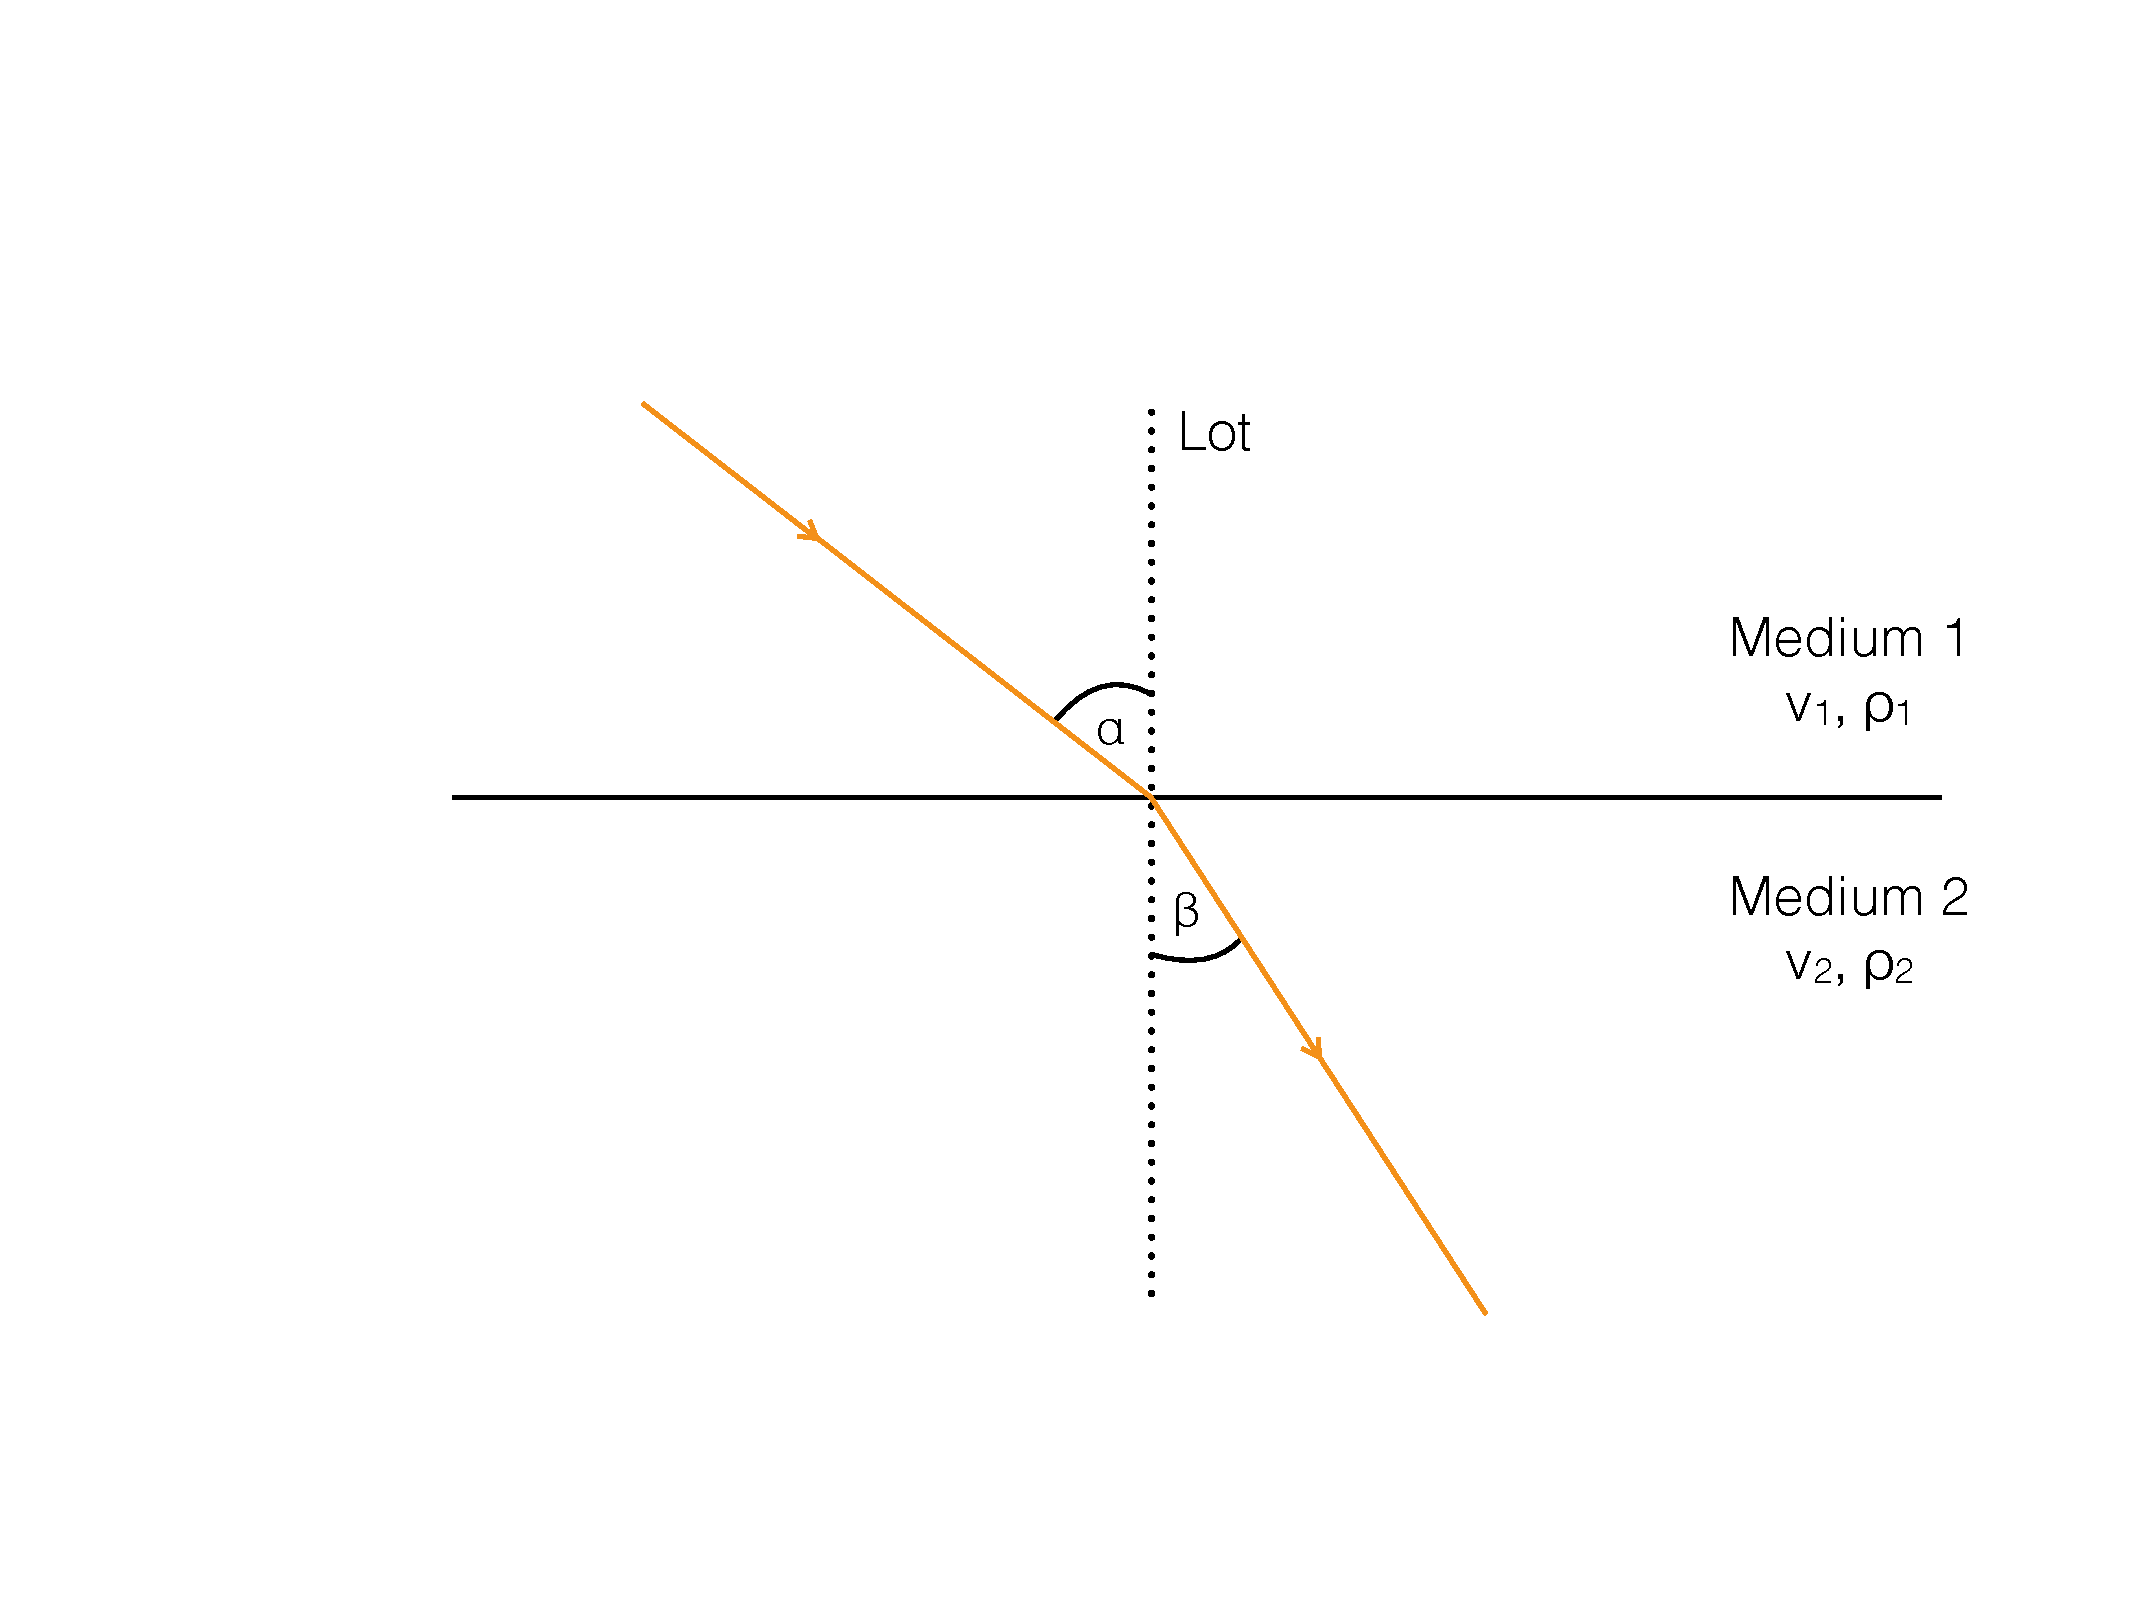
\includegraphics[scale=0.3]{SeismikBilder/Brechungsgesetz}
	\end{subfigure}
	\begin{subfigure}[m]{0.75\textwidth}
	\centering
		\[\begin{aligned}
			\frac{sin(\alpha)}{sin(\beta)} = \frac{v_1}{v_2}
		\end{aligned}\]
	\end{subfigure}
\end{figure}


Wir schauen uns noch die Herleitung dieses Gesetzes an. Als Hilfsmittel nehmen wir uns die Grafik von oben, die wir um einige Größen erweitern. 

\begin{figure}[H]
	\centering
	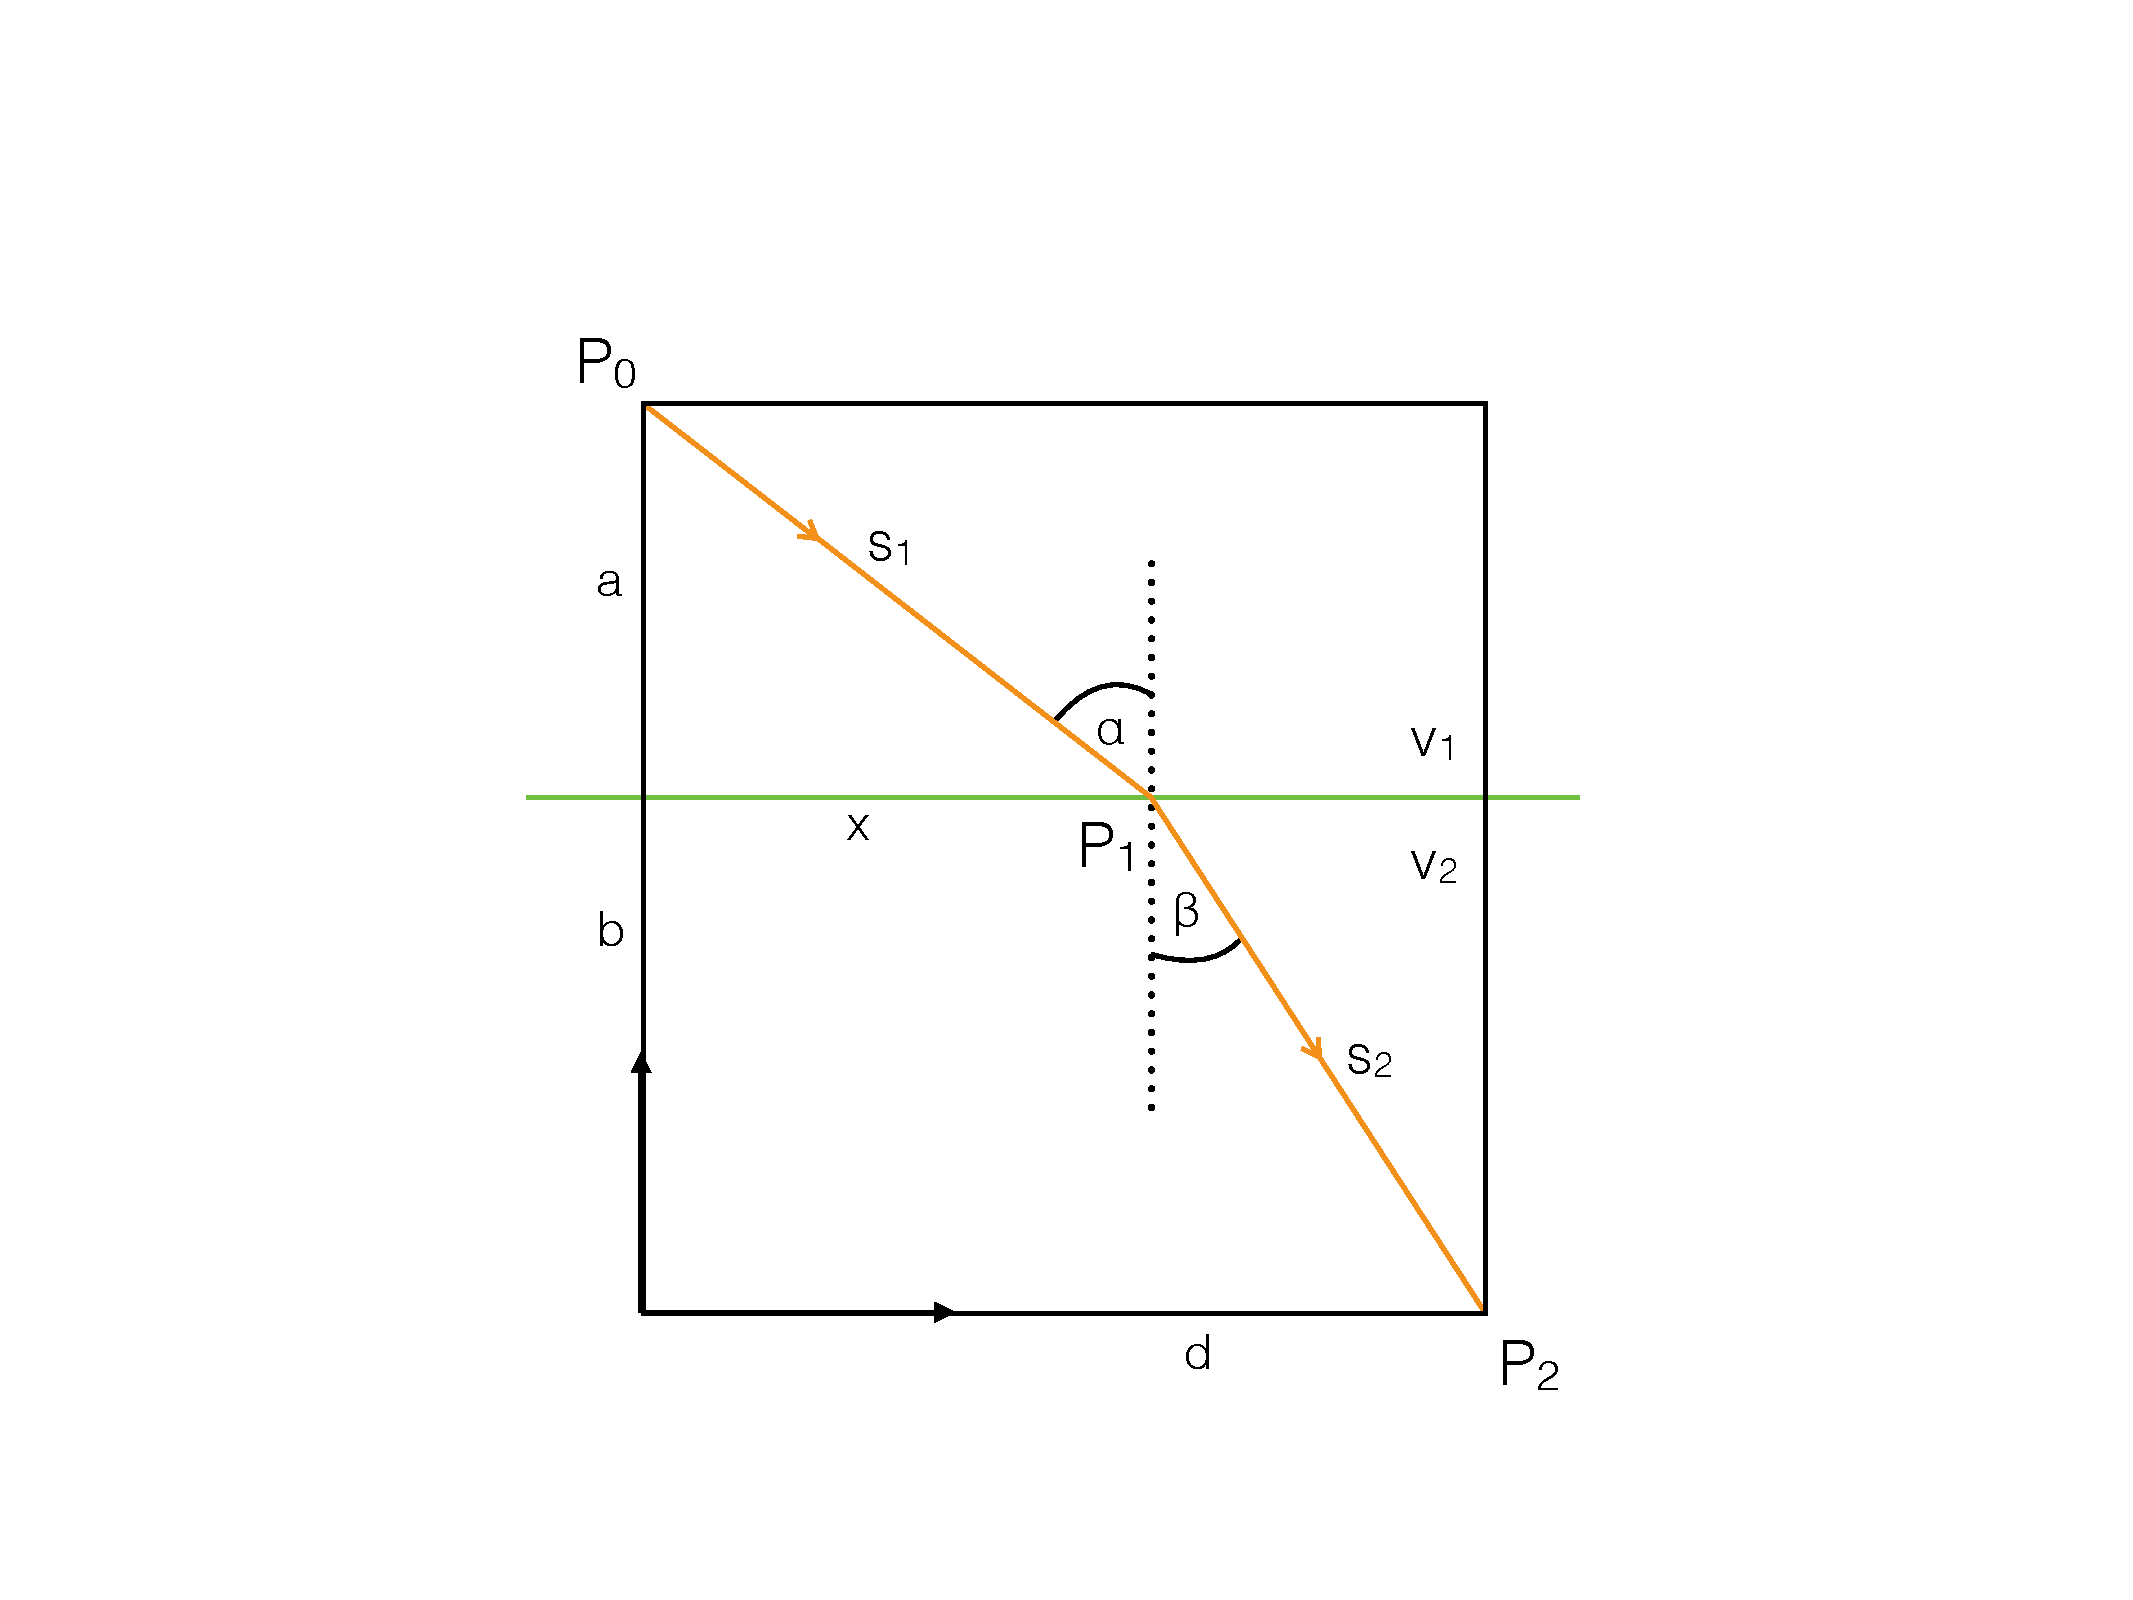
\includegraphics[scale = 0.5]{SeismikBilder/GrafikHerleitung}
\end{figure}
 
Eine Welle will immer den schnellsten Weg nehmen, also den Weg mit kürzester Laufzeit (\textbf{Fermat'sches Prinzip}).

Die Welle beginnt in unserem Beispiel bei $P_0 = \left( 0, \ a + b \right)$ und geht durch den Punkt $P_1 = \left( x, \ b \right)$ zu $P_2 = \left( d, \ 0 \right)$.

Im oberen Medium hat die Welle die konstante Geschwindigkeit $v_1$ und im Unteren $v_2$. Die Welle erfährt keine Beschleunigung. Aus diesem Grund können wir für die Berechnung der Laufzeit $t(x)$ der Welle den einfachen physikalischen Zusammenhang $s = v \cdot t$ verwenden. \begin{align*}
	t(x) = t_1 + t_2 = \frac{s_1}{v_1} + \frac{s_2}{v_2} = \frac{|P_1 - P_0|}{v_1} + \frac{|P_2 - P_1|}{v_2} = \frac{\sqrt{a^2 + x^2}}{v_1} + \frac{\sqrt{(d - x)^2 + b^2}}{v_2}
\end{align*}

Da wir die minimale Laufzeit suchen, leiten wir $t(x)$ ab und setzen diesen Term 0. \begin{align*}
	\frac{dt}{dx} = \frac{x}{  v_1 \cdot \sqrt{a^2 + x^2}} - \frac{(d - x)}{ v_2 \cdot \sqrt{(d - x)^2 + b^2}} \overset{!}{=} 0
\end{align*}

Wir betrachten erneut die Grafik und sehen: \begin{align*}
	x &= sin(\alpha) \cdot \sqrt{a^2 + x^2} \\
	d - x &= sin(\beta) \cdot \sqrt{(d - x)^2 + b^2}
\end{align*}

Daraus ergibt sich: \begin{equation*}
	0 = \frac{sin(\alpha)}{v_1} - \frac{sin(\beta)}{v_2}
\end{equation*} 
Und daraus wiederum das Brechungsgesetz \begin{equation*}
	\frac{sin(\alpha)}{sin(\beta)} = \frac{v_1}{v_2}
\end{equation*}

Mit dem Snellius'schen Brechungsgesetz lässt sich beispielsweise die bekannte Aussage "`Einfallswinkel = Ausfallswinkel"' leicht zeigen: 

\begin{figure}[H]
	\begin{subfigure}[m]{0.5\textwidth}
	\centering
		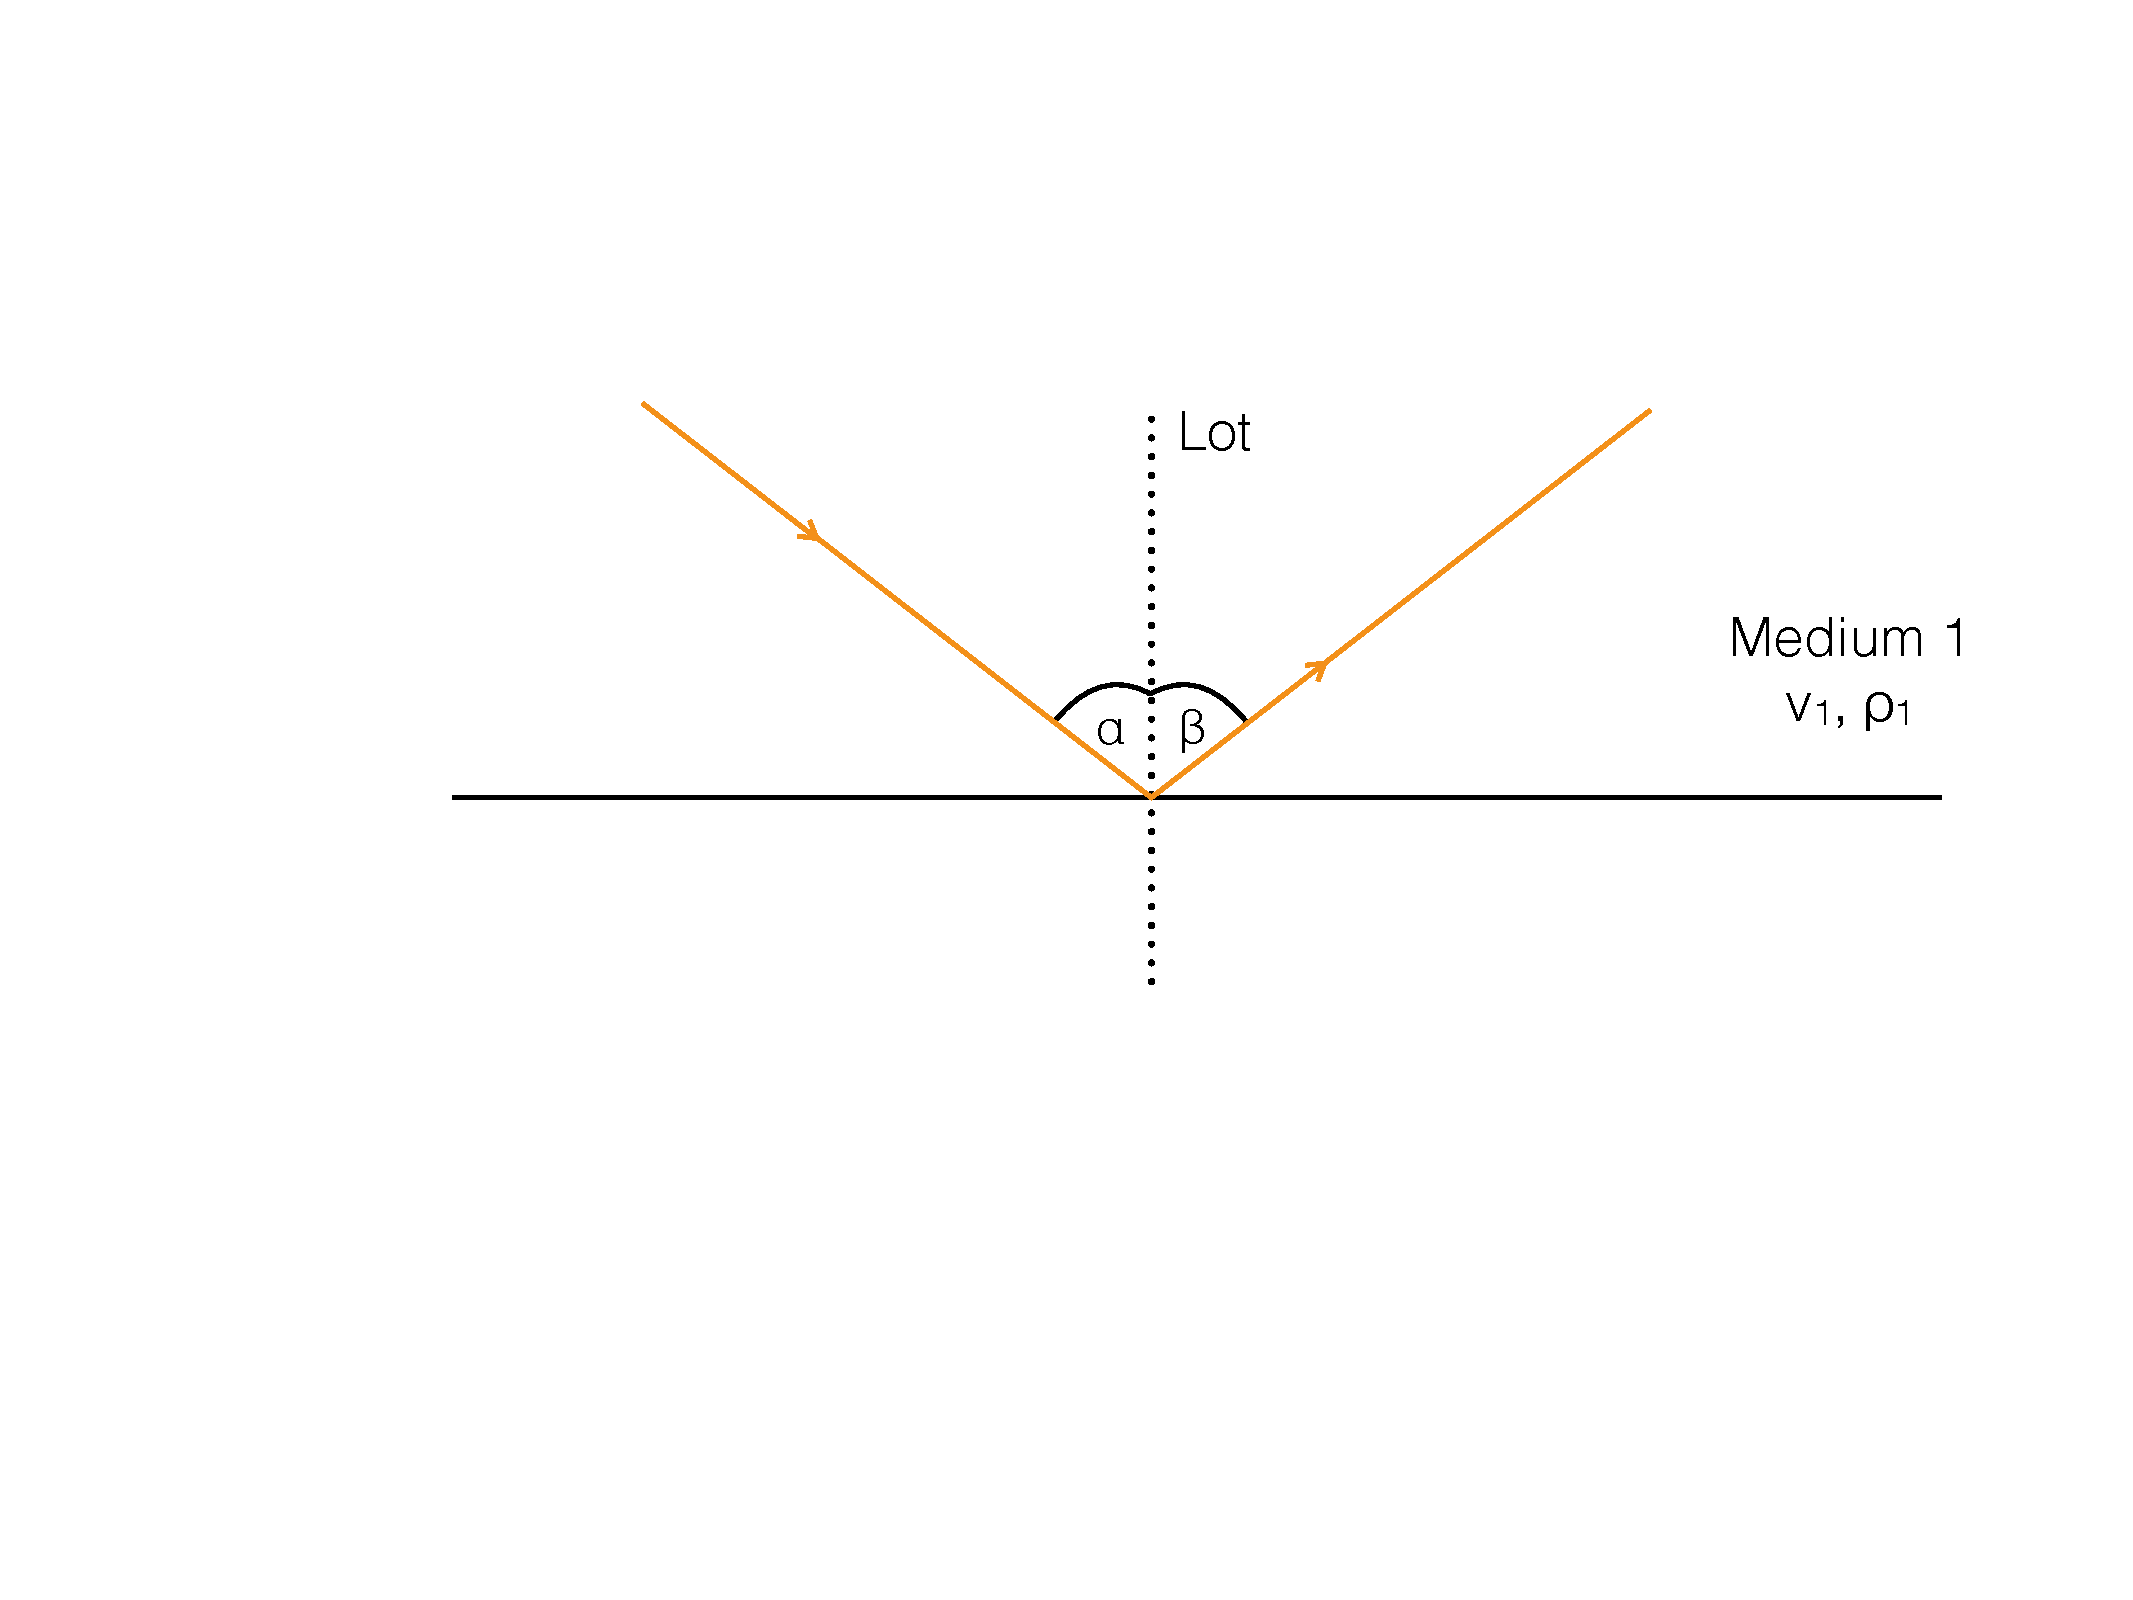
\includegraphics[scale=0.3]{SeismikBilder/EinfallsAusfallswinkel}
	\end{subfigure}
	\begin{subfigure}[m]{0.75\textwidth}
	\centering
		\[\begin{aligned}
			\frac{sin(\alpha)}{v_1} = \frac{sin(\beta)}{v_2} \\ \text{mit } v_1 = v_2 \quad \text{folgt } \alpha = \beta 
 		\end{aligned}\]
	\end{subfigure}
\end{figure}


\subsection{Reflexion und Transmission}
Die Streuwinkel der Welle nach Auftreffen auf die Grenzschicht für Reflexion und Transmission ergibt sich durch direkte Anwendung des Snellius'schen Brechungsgesetzes.

\begin{figure}[H]
	\centering
	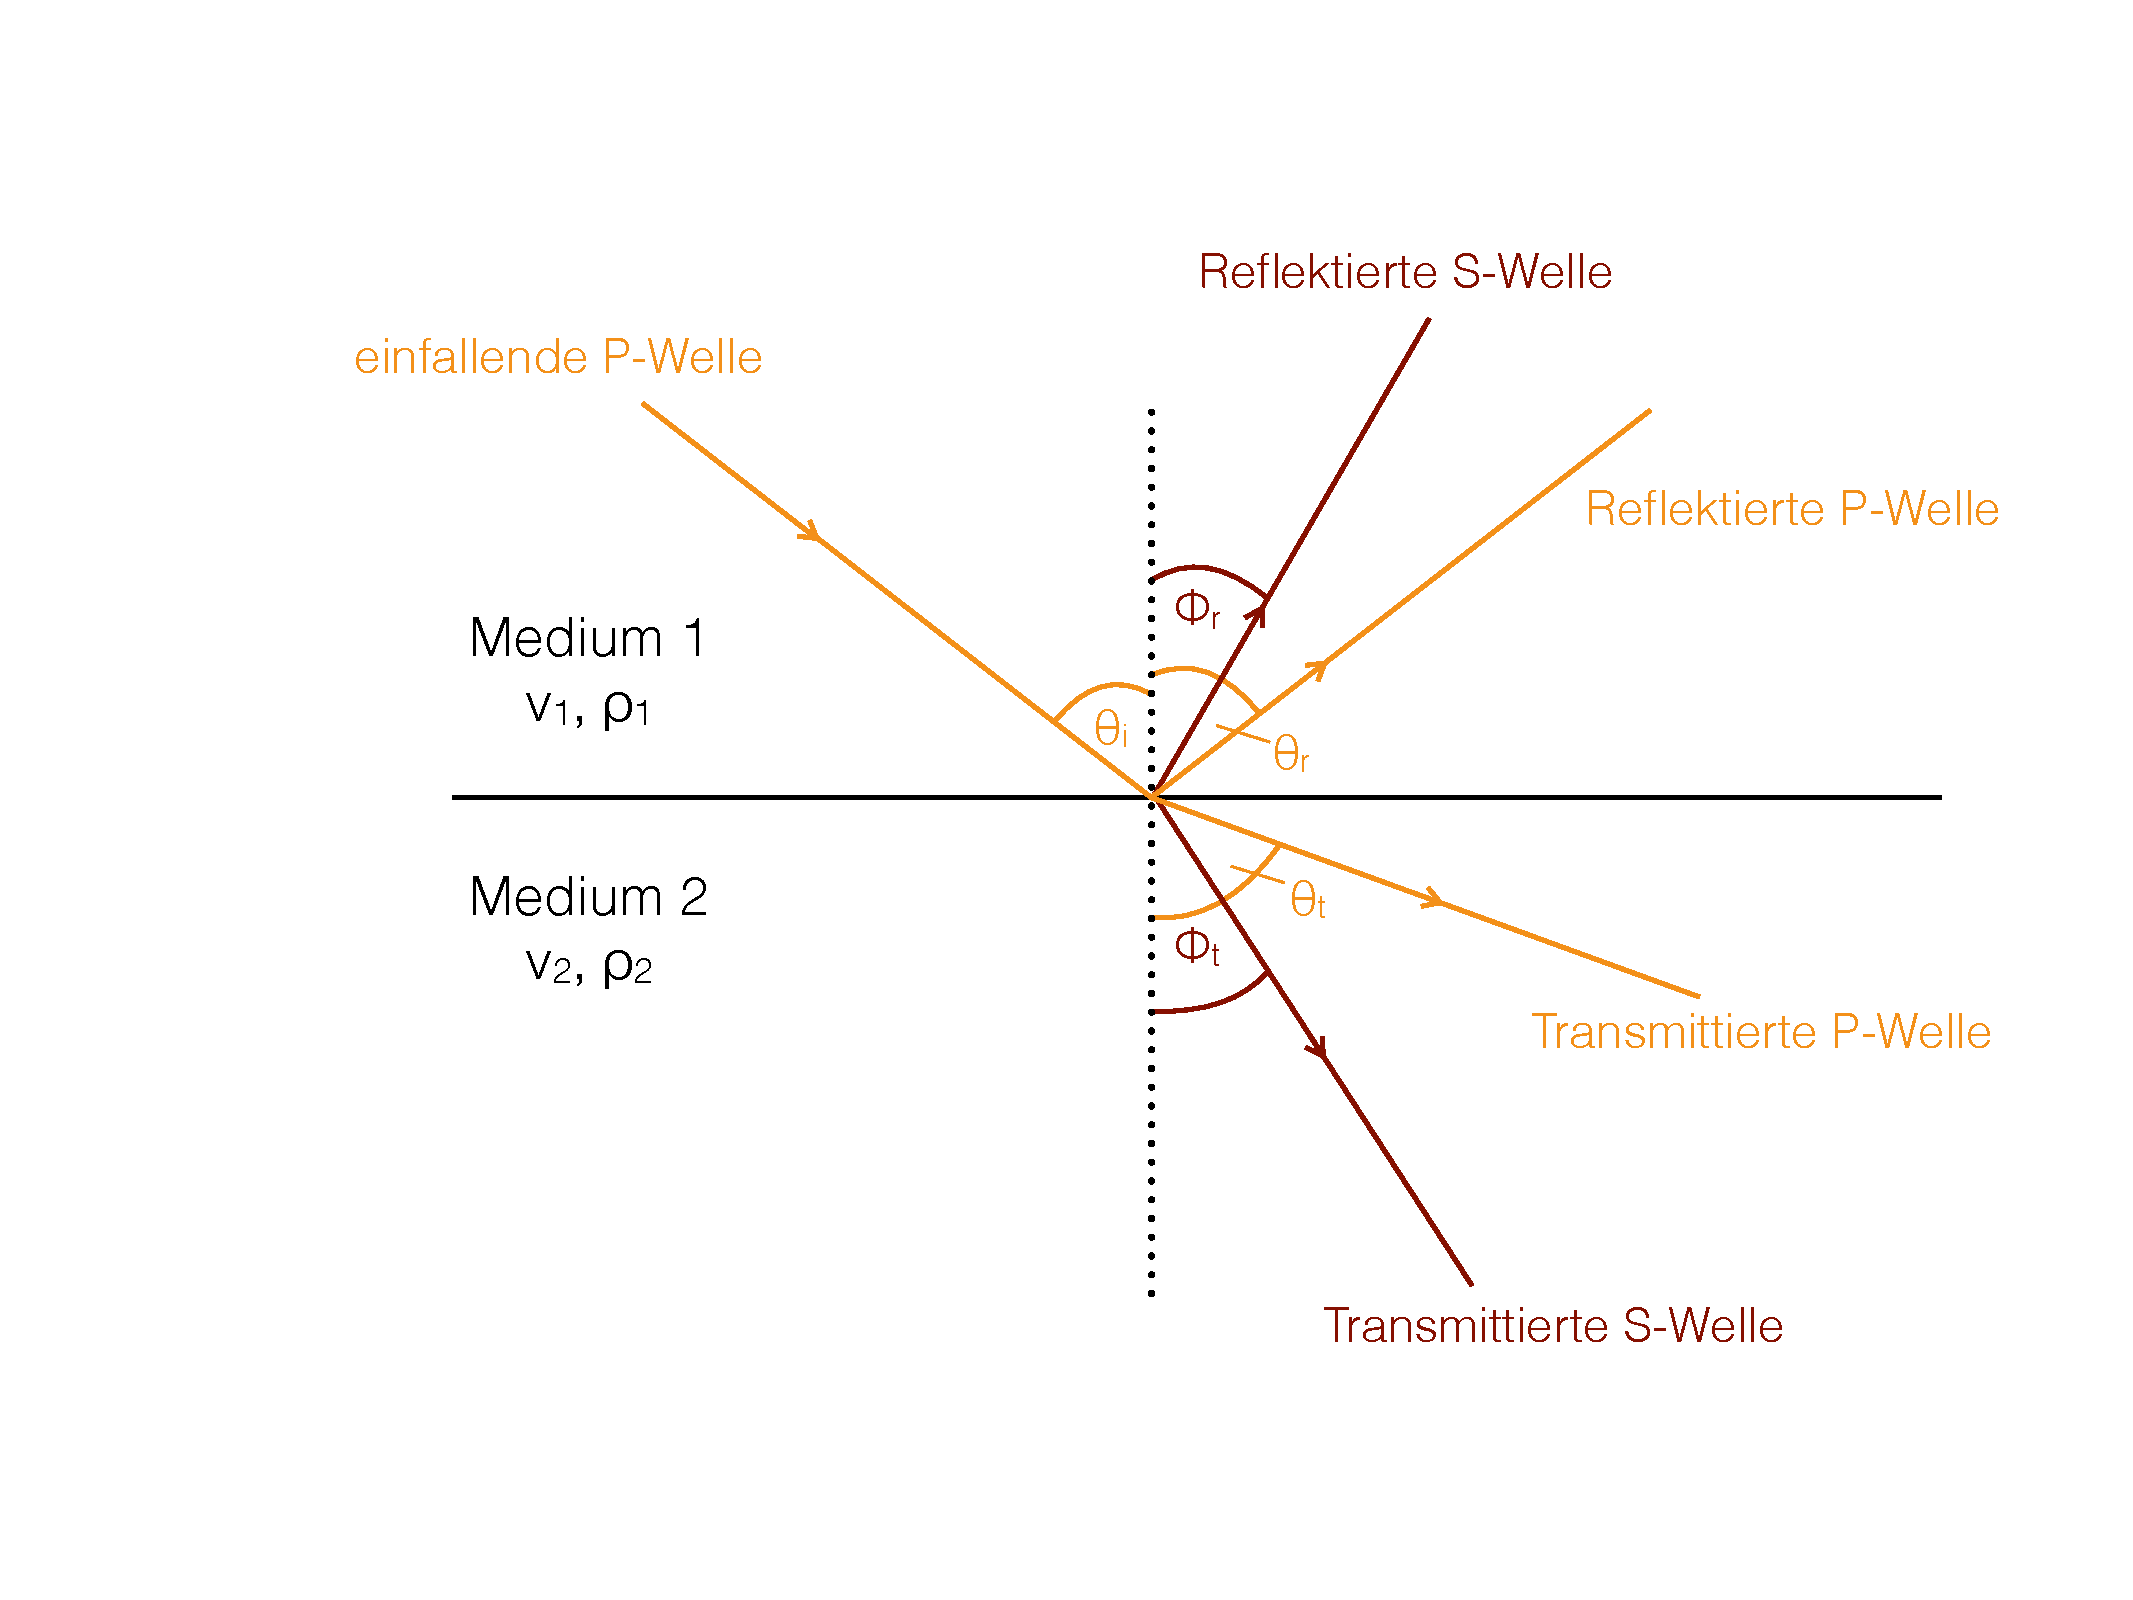
\includegraphics[width = \textwidth]{SeismikBilder/ReflexionTransmission}
\end{figure}

\begin{equation*}
	\frac{sin(\theta_{\text{i}})}{v_{\text{p}_1}} = \frac{sin(\theta_{\text{r}})}{v_{\text{p}_1}} = \frac{sin(\theta_{\text{t}})}{v_{\text{p}_2}} = \frac{sin(\phi_{\text{r}})}{v_{\text{s}_1}} = \frac{sin(\phi_{\text{t}})}{v_{\text{s}_2}}
\end{equation*}


\subsection{Refraktion und kritischer Winkel}
Auch die Refraktion lässt sich einfach mit Hilfe des Snellius'schen Brechungsgesetz berechnen.

\begin{figure}[H]
	\centering
	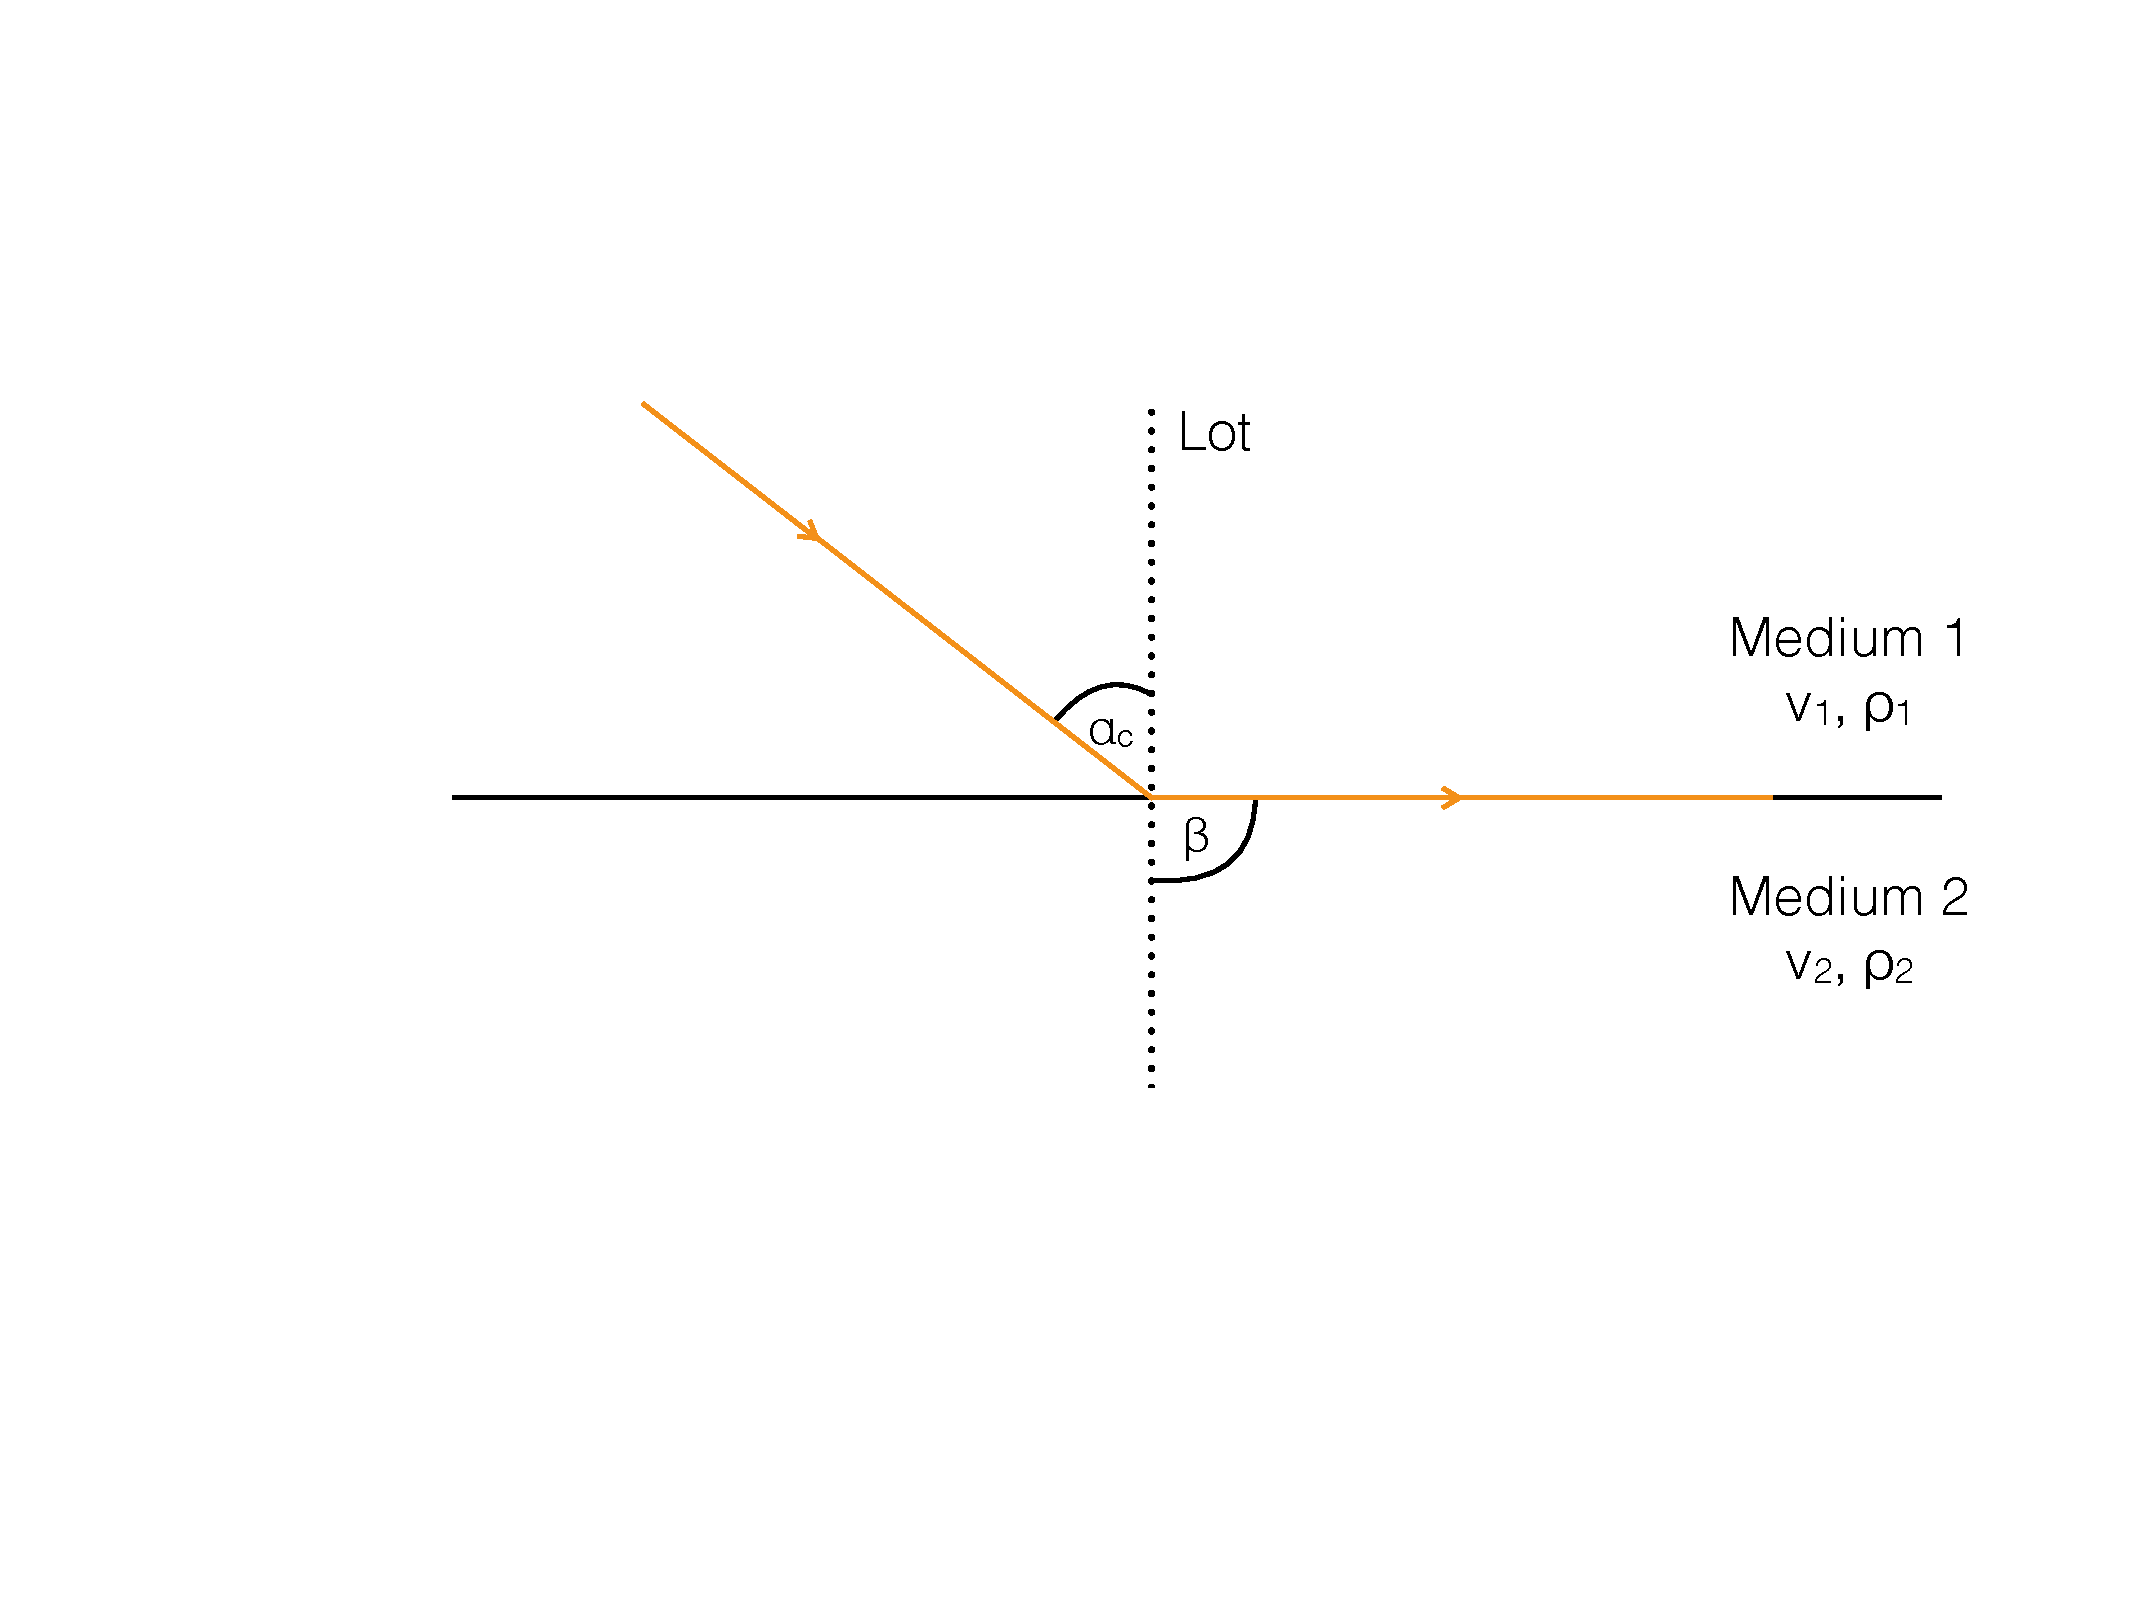
\includegraphics[width = \textwidth]{SeismikBilder/Refraktion}
\end{figure}

\begin{equation*}
	\frac{sin(\alpha)}{v_1} = \frac{sin(\beta)}{v_2} = \frac{1}{v_2} \quad \Rightarrow \quad sin(\alpha) = sin(i_c) = \frac{v_1}{v_2}
\end{equation*}
Dabei ist $i_c$ der \textbf{kritische Winkel}. Fällt die Welle unter dem kritischen Winkel auf die Schichtgrenze, wird die Welle also refraktiert und verläuft entlang der Grenze.


\subsection{Zusammenhang Brechungsgesetz und Wellengeschwindigkeit}
Bei jeder Gesteinsgrenze mit Übergang von einem weniger dichten zu einem dichteren Gestein nimmt die Ausbreitungsgeschwindigkeit einer seismischen Welle zu. Entsprechend ist eine Abnahme der Geschwindigkeit im umgekehrten Fall zu beobachten. Da die Dichte der Gesteine zum Erdinnern hin zunimmt, nimmt auch die Geschwindigkeit einer Welle entsprechend zu. Nach dem Snellius'schen Brechungsgesetz wird eine seismische Welle also mit zunehmender Tiefe vom Lot weg gebrochen. Je näher sie wieder an die Erdoberfläche kommt demnach zum Lot hin gebrochen. Dies erklärt den typischen bogenförmigen Verlauf einer seismischen Welle. Erreicht eine solche Welle wieder die Erdoberfläche, wird sie \textbf{Tauchwelle} genannt.


\begin{figure}[H]
	\centering
	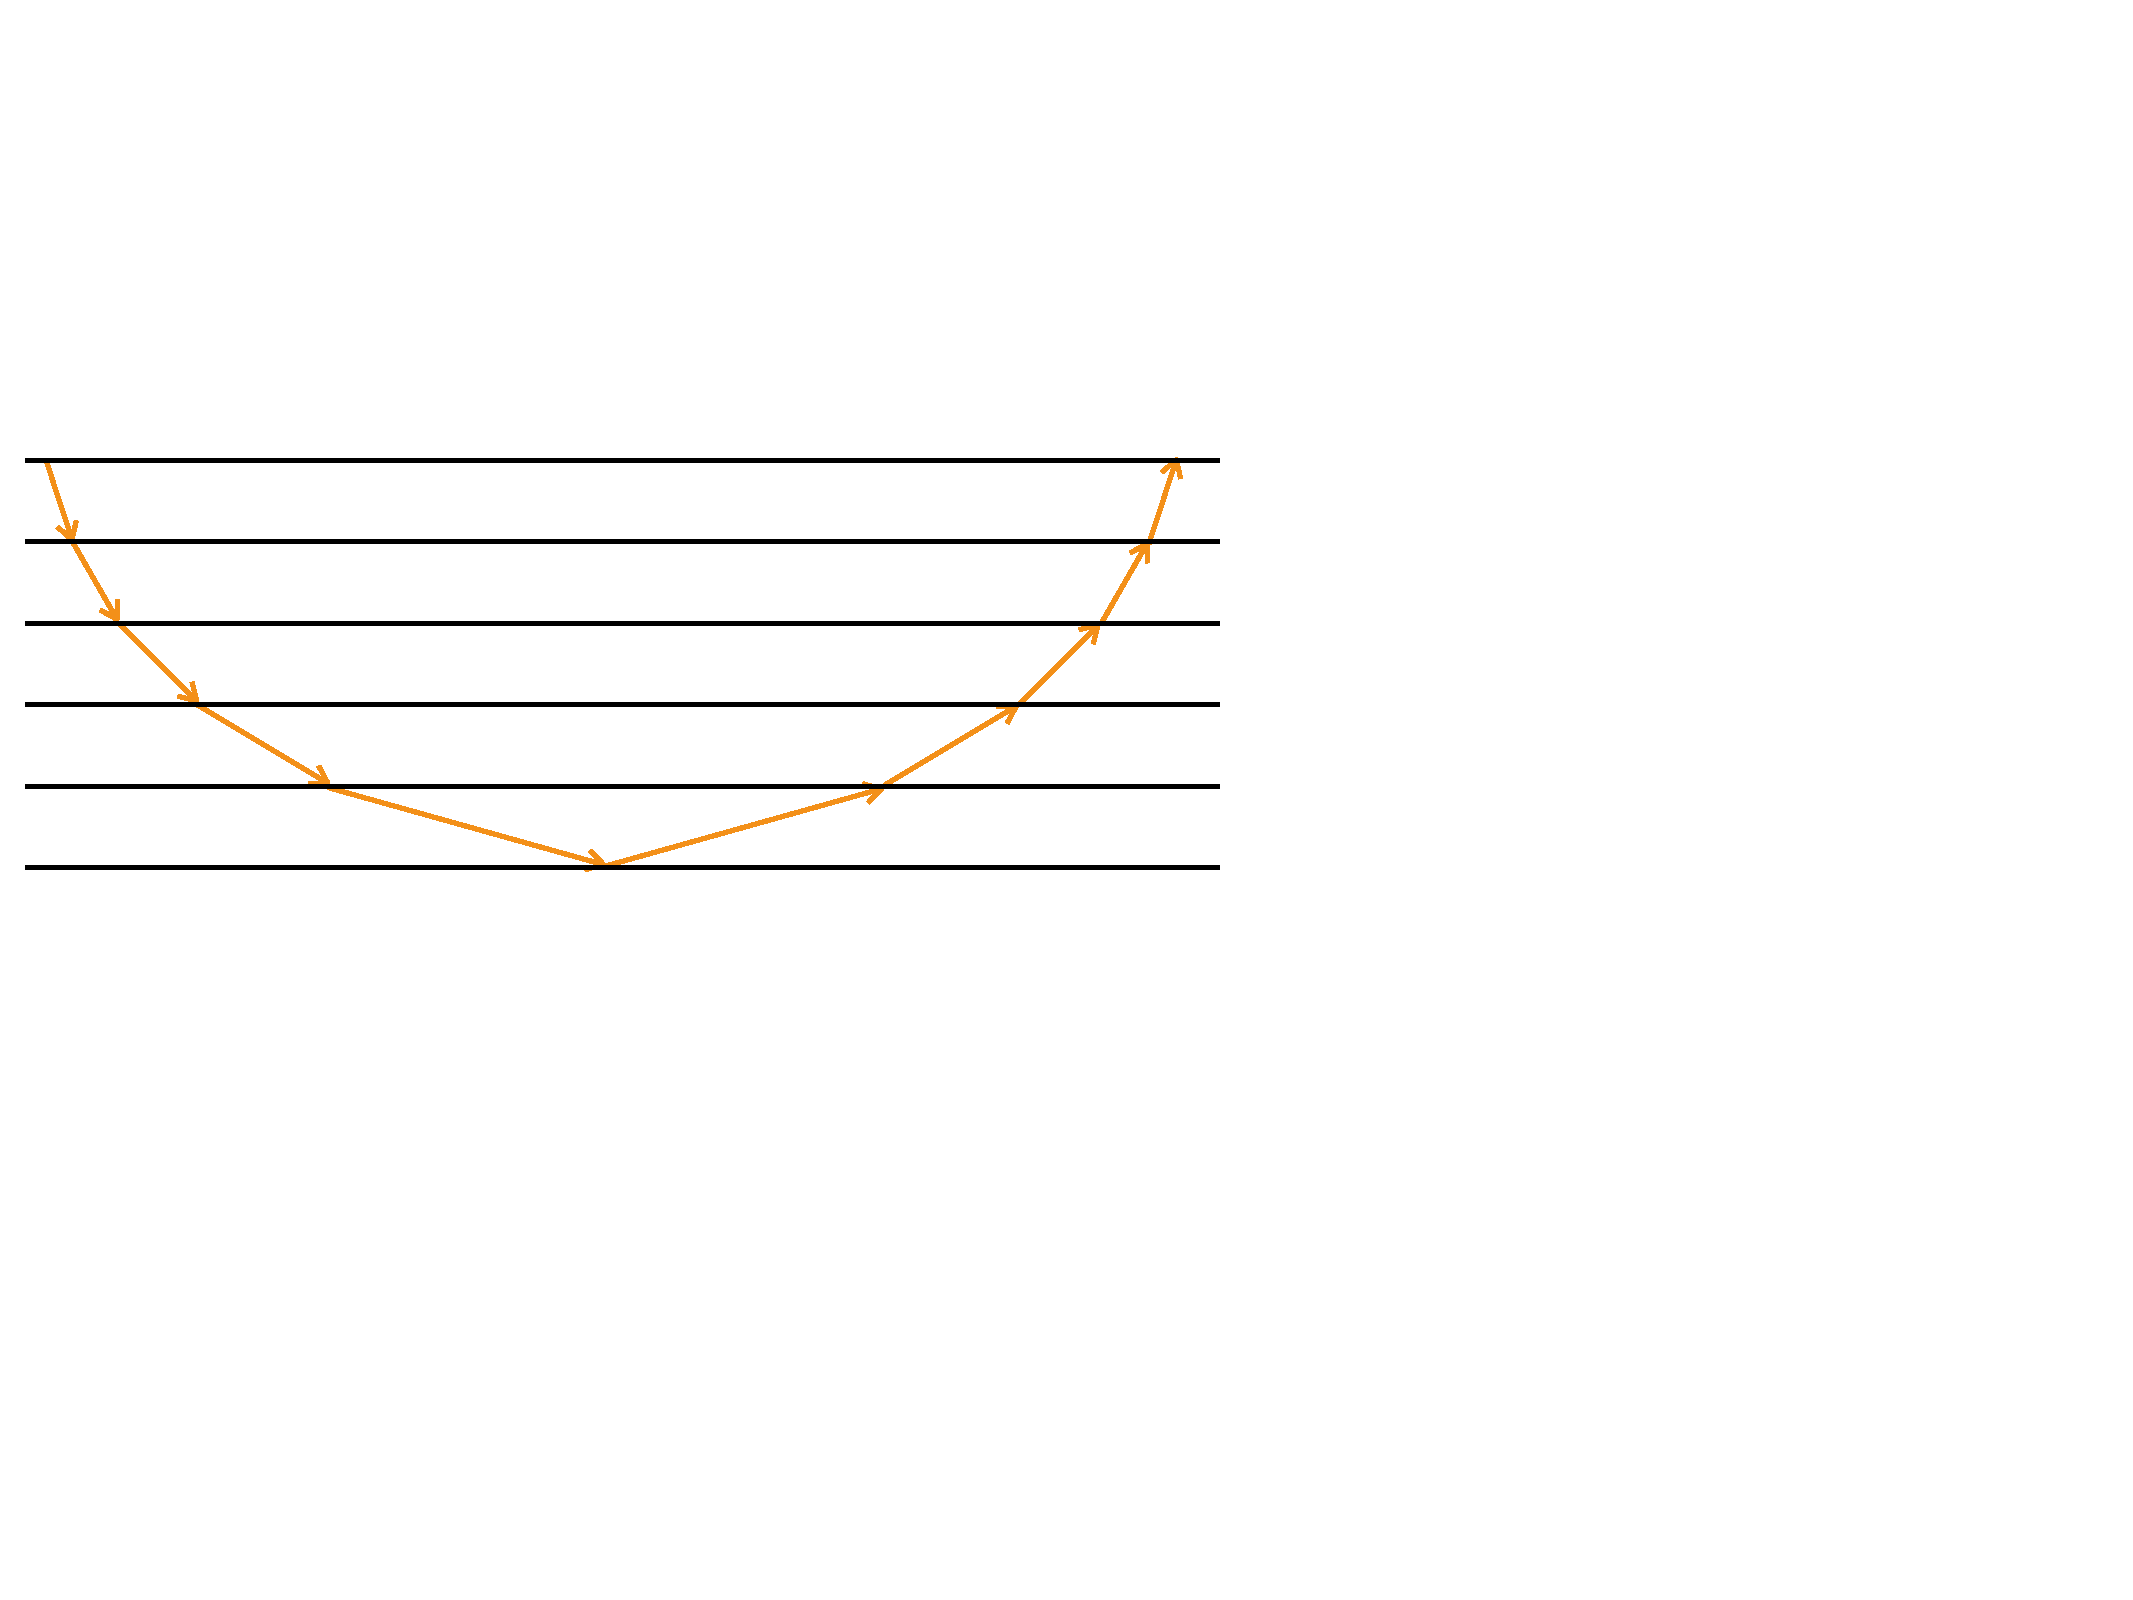
\includegraphics[width = \textwidth]{SeismikBilder/Tauchwelle}
\end{figure}


\section{Zeitmittelgleichung}
In der seismischen Geophysik ist die Lauftzeit und damit die Geschwindigkeit einer Welle im Untergrund sehr wichtig. Bei den obigen Berechnungen sind wir davon ausgegangen, dass die einzelnen Schichten homogen sind. Dies lässt sich aber nicht immer so annähern. 

Eine Möglichkeit, die Geschwindigkeiten abzuschätzen, ist die Zeitmittelgleichung. Diese verrechnet die einzelnen Materialgeschwindigkeiten aus denen sich der Untergrund zusammensetzt. 

Um diese Gleichung aufstellen zu können, wird ein vereinfachtes Gesteinsmodell angenommen: 

\begin{figure}[H]
	\centering
	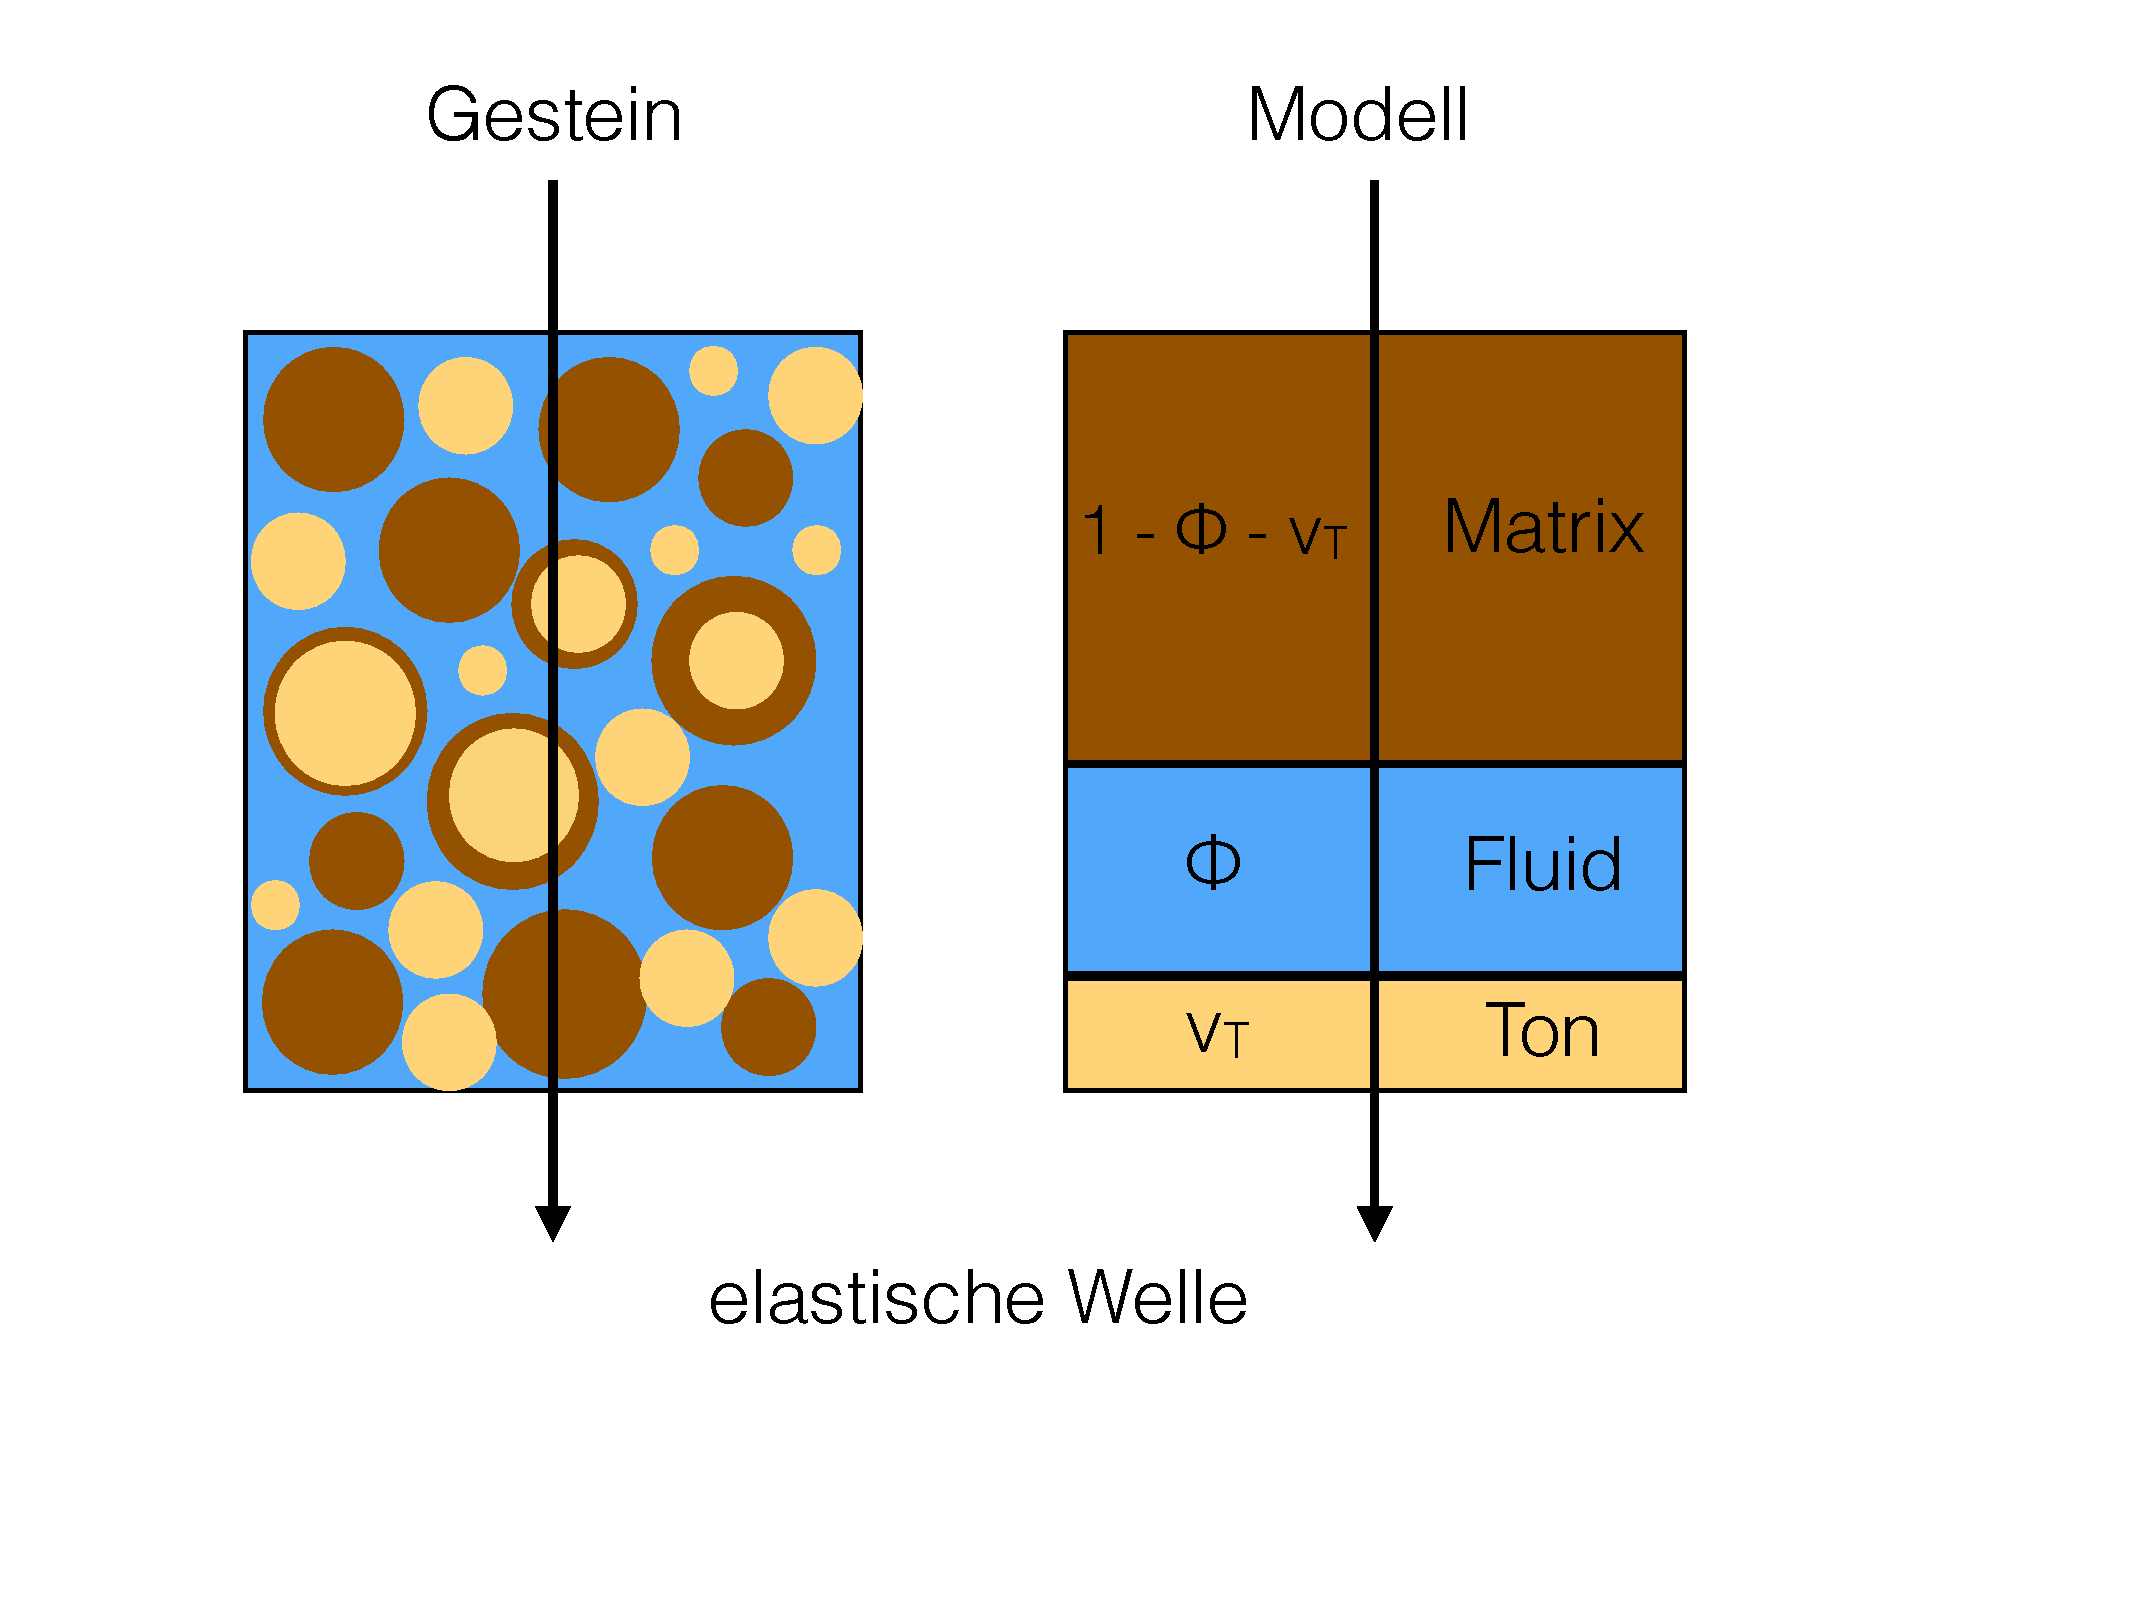
\includegraphics[width = \textwidth]{SeismikBilder/Zeitmittelgleichung}
\end{figure}

\begin{itemize}
	\item volumenproportionale, ebene Platten für jeden Bestandteil
	\item keine Wechselwirkungen zwischen den Materialien
	\item Tonkorrektur
\end{itemize}

Die Zeitmittelgleichung ergibt sich aus der Laufzeitgleichung der Welle \begin{equation*}
	T = T_{\text{Matrix}} + T_{\text{Fluid}} + T_{\text{Ton}}
\end{equation*}

Da die Laufzeit $T$ umgekehrt propotional zu $1/v$ ist, ergibt sich: \begin{equation*}
	\frac{1}{v_{\text{eff}}} = \frac{1 - \phi - v_{\text{T}}}{v_{\text{Matrix}}} + \frac{\phi}{v_{\text{Fluid}}} + \frac{v_{\text{T}}}{v_{\text{Ton}}}
\end{equation*}

\begin{tabular}{ll}
	$v_{\text{eff}}$ & effektive Ausbreitungsgeschwindigkeit im Gestein \\
	$v_{\text{Matrix}}$ & mittlere Ausbreitungsgeschwindigkeit in den Matrixbestandteilen \\
	$v_{\text{Fluid}}$ & mittlere Ausbreitungsgeschwindigkeit in den Fluiden/Gasen \\
	$v_{\text{Ton}}$ & mittlere Ausbreitungsgeschwindigkeit in den Tonbestandteilen \\
	$\phi$ & Porosität (relativer Volumenanteil der Gase/Fluide) \\
	$1 - \phi - v_{\text{T}}$ & relativer Volumenanteil der Matrix \\
	$v_{\text{T}}$ & relativer Volumenanteil des Tons
\end{tabular}

\section{Ausblick}
Seismische Wellen lassen sich für geophysikalische Messungen nutzen. Sie werden durch beispielsweise einen Hammerschlag auf die Erdoberfläche (\textbf{Hammerschlagseismik}) künstlich erzeugt und mit speziellen Messgeräten (\textbf{Geophone}) gemessen. Die gemessenen Daten lassen Rückschlüsse auf die Struktur des Untergrundes zu. Die nächsten beiden Kapitel beschäftigen sich mit zwei verschiedenen Messverfahren auf Grundlage der Seismik.  





